\documentclass[11 pt]{report}

% Typography packages
\usepackage{microtype}
\usepackage[T1]{fontenc}
\usepackage{inconsolata}
\usepackage{fourier}
\usepackage{setspace}
\usepackage{textcomp}
\usepackage{booktabs}

% Math packages
\usepackage{amssymb}
\usepackage{amsmath}
\usepackage{bm} % Bold Greek math

% Figure and captioning packages
\usepackage[export]{adjustbox}
\usepackage[margin=0.1\textwidth]{caption} % Adjust caption text column margins
\usepackage{subcaption} % Subfigures with subcaptions
\usepackage{wrapfig} % Text wrapping around figures
\usepackage[export]{adjustbox} % Fine-tuned figure placement
\usepackage{float} % Control positioning of figures

% Algorithm packages
\usepackage{algorithm} % Algorithm environment
\usepackage{algorithmicx} % Improvements to Algorithm environment
\usepackage[noend]{algpseudocode} % No "end" statement at the end of an algorithm

% Other miscellaneous packages
\usepackage{array} % For fixed-length tables
\usepackage{graphicx}
\usepackage{hyperref}
\usepackage{todonotes} % DELETE WHEN FINISHED
\usepackage{verbatim} % DELETE WHEN FINISHED

\linespread{1.15}

\hypersetup{
    pdffitwindow=false,     % window fit to page when opened
    pdfstartview={FitH},    % fits the width of the page to the window
    pdftitle={Joshua Eddy MS Thesis},    % title
    pdfauthor={Joshua Eddy},     % author
    pdfnewwindow=true,      % links in new PDF window
    colorlinks=true,       % false: boxed links; true: colored links
    linkcolor=black,          % color of internal links (change box color with linkbordercolor)
    citecolor=black,        % color of links to bibliography
    filecolor=magenta,      % color of file links
    urlcolor=blue           % color of external links
}

% Control vertical spacing within matrices
\makeatletter
\renewcommand*\env@matrix[1][\arraystretch]{%
  \edef\arraystretch{#1}%
  \hskip -\arraycolsep
  \let\@ifnextchar\new@ifnextchar
  \array{*\c@MaxMatrixCols c}}
\makeatother

% Control the margins on block quotes
\newenvironment{myquote}[1]%
  {\list{}{\leftmargin=#1\rightmargin=#1}\item[]}%
  {\endlist}
  
\renewcommand{\arraystretch}{1.2}

\begin{document}

\thispagestyle{empty}

\begin{center}
{\Large 
A Hardware-Minimal Unscented Kalman Filter Framework for Visual-Inertial Navigation of Small Unmanned Aircraft
}
\vfill

Joshua Galen Eddy

\vfill

Thesis submitted to the Faculty of the \\
Virginia Polytechnic Institute and State University \\
in partial fulfillment of the requirements for the degree of

\vfill

Master of Science \\
in \\
Aerospace Engineering

\vfill

Kevin Kochersberger, Chair \\
Mazen Farhood \\
Craig Woolsey

\vfill

May 5, 2017 \\
Blacksburg, Virginia

\vfill

Keywords: Unscented Kalman Filter, SLAM, State Estimation, Localization,\\
Visual-Inertial Navigation, Unmanned Aircraft
\\
Copyright 2017, Joshua Galen Eddy
\end{center}

\pagebreak
\pagenumbering{roman}
\chapter*{Abstract}

\pagenumbering{roman}

This thesis presents the formulation and implementation of an Unscented Kalman Filter (UKF) framework for fusion of visual and inertial sensors in unmanned aircraft navigation. Specifically, we fuse sensor readings from a 3-axis accelerometer, 3-axis gyroscope, and a Simultaneous Localization and Mapping (SLAM) algorithm to estimate the pose of an aircraft, such as a quadcopter, capable of hovering flight. We discuss the formulation of our UKF fusion algorithm, the development of a Robot Operating System (ROS) software package implementing the algorithm, and several experiments in which this algorithm was used to track the motion of a physical vehicle simulating hovering flight in an indoor environment. We verify the filter's effectiveness by comparing its output to that of a Vicon motion capture system. We then discuss possible applications of this system and future work which may build upon the results developed herein.
\chapter*{Acknowledgments}

This work would not have been possible were it not for my graduate adviser and committee chair, Dr.~Kevin Kochersberger. He has been a constant source of support since October 2012 when he provided my friends and me with lab space in which to design our first competition robots. Over the ensuing five years, Dr.~Kochersberger has played a pivotal role in my development as an engineer and researcher. He demonstrates his commitment to nurturing students every day by giving tirelessly of his time and energy.

It is also my pleasure to thank Dr.~Danette Allen of the NASA Langley Autonomy Incubator (now the Intelligent Flight Systems and Autonomy Innovation Laboratory), who provided me with two summer internships in her lab and taught me much of what I know today about Kalman filtering. Dr.~Allen supplied me with both funding and equipment in order to perform this research, even going so far as to allow me to use her lab's motion capture facilities for my experiments.

I would also like to thank Dr.~Loc Tran and Mr.~James Neilan of NASA Langley and Ralph Williams of Analytical Mechanics Associates, who collectively provided me with hours of programming guidance during my time at the Autonomy Incubator.

Special thanks go to Samuel Rubenking, who stuck with me to the end. Thanks, Sam.
\tableofcontents
\listoftables
\listoffigures
\chapter*{Acronyms}

\begin{description}
\item [AR] Augmented Reality
\item [EKF] Extended Kalman Filter
\item [GPS] Global Positioning System
\item [KF] Kalman Filter
\item [IMU] Inertial Measurement Unit
\item [MSF-EKF] Multi-Sensor Fusion Extended Kalman Filter
\item [PTAM] Parallel Tracking and Mapping
\item [SLAM] Simultaneous Localization and Mapping
\item [ROS] Robot Operating System
\item [UAS] Unmanned Aircraft System
\item [UAV] Unmanned Aerial Vehicle
\item [UKF] Unscented Kalman Filter
\item [UT] Unscented Transform
\item [UTM] Unmanned Traffic Management
\item [VIN] Visual-Inertial Navigation
\item [VO] Visual Odometry
\end{description}
\pagebreak

\pagenumbering{arabic}
\chapter{Introduction}

Until recently, the sensing and localization capabilities of small unmanned aerial vehicles (UAVs) have been computationally constrained due to restrictions on both the size and weight of sensors and onboard computer systems. Recent advances in miniaturized desktop computers, as well as low-power Graphics Processing Units (GPUs), have enabled a new class of computationally intensive algorithms to run onboard small aircraft without degrading flight time or other performance metrics. Specifically, small drones now present a viable platform for high-fidelity Simultaneous Localization and Mapping (SLAM), visual object recognition, and state estimation algorithms employing numerous heterogeneous sensors. In addition, the rising popularity of drones among hobbyists and researchers has fueled tremendous growth in the markets for brushless motors, electronic speed controllers, and airframes. With high-quality flight hardware and lightweight computers readily available, the arsenal of the robotics researcher has never been better stocked. The work detailed in this thesis is, in many ways, the product of these advantageous market conditions. With small aircraft capable of lifting heavier payloads and computers now lighter and smaller in footprint, demand is high for outfitting high-performance vehicles with top-notch sensing capabilities.

This work centers on an algorithm known as the Unscented Kalman Filter (UKF), a sensor fusion method for estimating the state of systems such as small aircraft. For years, this algorithm was inaccessible to roboticists and aerospace researchers alike due to its computational complexity. Computers capable of running the algorithm were simply too large, too heavy, and too power-hungry to be viable onboard components of small UAVs. The advent of smaller computers has changed this state of affairs. In this thesis, we present a formulation of the Unscented Kalman Filter aimed at estimating the pose of a quadcopter. This UKF formulation fuses outputs from only two sensors: an inertial measurement unit (IMU) and a downward-facing monocular camera. These two data streams are fused to estimate the vehicle's pose in real time. We propose this UKF framework as a hardware-minimal starting point for advanced multi-sensor fusion in UAV navigation.

\subsection{System Applications}

Applications for this system are wide-ranging, spanning virtually every conceivable use for a small drone. The following is a non-exhaustive list of possible applications:
\begin{enumerate}
    \item Mapping and 3D reconstruction of structures and topography,
    \item Emergency response,
    \item Infrastructure inspection,
    \item Autonomous package delivery, and
    \item Military/defense solutions.
\end{enumerate}
What all of these applications have in common is the need for robust localization. In each of the above scenarios, losing GPS could cause a crash. In such an event, the vehicle itself would pose a real threat to bystanders and property. Moreover, in the case of military aircraft, the vehicle could be captured by hostile forces.

\subsubsection{Mapping and 3D Reconstruction}

Growing demand for so-called ``precision agriculture'' has brought with it the need to map large areas of cropland at a high speed, with a low cost point. In the past, this need has been met by using satellite imagery and human-captured photography. With the arrival of low-cost drones, this work has been offloaded to aerial robots. Outfitted with specialized sensors such as hyperspectral cameras\footnote{\url{https://en.wikipedia.org/wiki/Hyperspectral_imaging}}, small UAS are now able to provide minute-by-minute coverage of large expanses of land. More interesting still, these robots can be outfitted with reservoirs of pesticide or fertilizer and deployed to spray individual plants autonomously. It is in roles such as this that high-accuracy robust localization becomes a necessity. The accuracy required for precision agriculture can be provided by utilizing the sensor fusion techniques discussed in this thesis.

The surfaces of buildings and other structures can be mapped in a similar fashion, given the appropriate sensors and the right framework by which to fuse them. 3D reconstruction has become popular among real estate agents, safety inspectors, and other parties with a vested interest in precise 3D renderings of large geometries. In this case, the aircraft must be able to localize itself precisely in order to take full advantage of onboard sense-and-avoid technologies. The ability of the aircraft to estimate its position is crucial to its ability to map hard-to-reach areas and maintain stable flight. Sensor fusion systems shine when GPS and other sensors are inevitably compromised by various environmental factors.

\subsubsection{Emergency Response}

UAS technologies have become a desirable tool for first responders in many parts of the world. The ability to deploy a UAV to survey forest fires or search for missing persons has been a game changer for law enforcement and emergency response teams. In the case of looking for survivors of a natural disaster, the requirements for an effective vehicle system are accurate localization and overall robustness. Vehicles sent into disaster areas will have to be able to navigate in sensor-compromising environments, sometimes at substantial speed. This use case highlights the need for redundant sensors and intelligent, failure-resistant sensor fusion.

\subsubsection{Infrastructure Inspection}

Infrastructure inspection is similar in several respects to 3D mapping. In both cases, small drones are preferable to manned aircraft because of their low cost, high maneuverability, and ease of use. In recent years, governments and private corporations have taken an interest in using small aircraft to automate the inspection of many types of infrastructure, including the following:
\begin{enumerate}
    \item Power lines,
    \item Oil rigs,
    \item Gas pipelines,
    \item Railroads, and
    \item Buildings.
\end{enumerate}
UAVs are an obvious ally to companies servicing most types of static infrastructure. Inspecting miles of wires or railroad track is a task well-suited to today's UAVs, which commonly ship with intuitive flight planning software. Operators---even those who have no experience flying remote-control aircraft---are now able to program missions and deploy drones with ease. The aircraft are able to survey miles of infrastructure regardless of conditions on the ground, such as flooding, ill-maintained roads, or wild animals. Operators with First-Person View (FPV) hardware can watch video streaming live from the aircraft as if they were onboard themselves. The need for robust localization here is obvious: the UAV cannot inspect anything to which it cannot navigate. Operating in the wilderness may require flying below the forest canopy or under natural overhangs that could block GPS reception. The same is true in urban environments, where tall buildings create so-called ``urban canyons'' which compromise GPS effectiveness. Large metal structures can also distort magnetometry readings and thus undermine the aircraft's ability to maintain its heading. In any case, UAVs used for large-scale inspections will be dependent upon intelligently combined sensing modalities.

\subsubsection{Autonomous Package Delivery}

A number of organizations, most notably Amazon\footnote{\url{https://www.amazon.com/Amazon-Prime-Air/b?node=8037720011}}, have made big bets on drones as the future of delivery services. The task of delivering goods to individual homes is no trifling matter. American homes come in all shapes and sizes and are surrounded by numerous structures and natural obstacles that could endanger a delivery aircraft and, by extension, the people and property nearby. Moreover, any drone delivery service would have to be predicated upon the ability of the UAV to land with sub-meter accuracy. Delivery drones will have to land precisely in cluttered environments amid dynamic obstacles. Visual sensing will be extremely important for identifying safe landing zones, avoiding power lines and fences, and surmounting other environmental challenges. GPS alone will not be enough to guide the vehicle safely in every conceivable circumstance. 

\subsubsection{Military/Defense Solutions}

Perhaps the most obvious application of a UKF fusion framework is in military operations, where precision navigation and robustness to sensor degradation are paramount for protecting soldiers in the field. As of the time of this writing, UAVs have been used in combat for years. However, augmented navigation could still make revolutionary contributions in areas such as
\begin{enumerate}
    \item Robust tracking of friendly and hostile elements,
    \item Remote observation of roads and vehicle-related hazards,
    \item Autonomous deliveries of materiel in-theater, and
    \item Human-machine teaming.
\end{enumerate}
Every combat zone will constitute a hostile environment for UAV operations, especially in the presence of GPS spoofing/jamming technologies. Combat UAVs will have to be able to tolerate multiple simultaneous sensor failures. Moreover, in-theater urban flight operations bring with them all of the same difficulties mentioned above, but with the added challenge of violent enemy interdiction. Robust sensor fusion could automate the task of operational overwatch and provide mission-critical intelligence in a timely manner---but only if the vehicle can localize itself reliably in sensor-hostile environments.

\section{Personal Motivation}

\textit{This section is largely comprised of background information regarding certain experiences leading up to, and motivating, the research developed in my thesis. This section does not contain any technical material, and is included only to provide context to the larger work.}

\vspace{1em}

\begin{wrapfigure}{r}{0.4\textwidth}
  \centering
    
\includegraphics[width=0.4\textwidth]{CARD_gearREALLYBIG}
  \caption[CARD Team Logo]{The CARD team logo.}
  \label{fig:card_logo}
\end{wrapfigure}

I first took an interest in unmanned aircraft in the fall of 2012, my sophomore year of college. Several of my friends and I founded the Cooperative Autonomous Robotics Design (CARD) team at Virginia Tech in order to pursue our shared interest in autonomous vehicles. Our core team consisted of a dozen students devoted to designing and competing with drones and other robotic vehicles. Our team, guided by my future graduate adviser, Dr.~Kevin Kochersberger, entered two design competitions and brought home two awards for the university. We were also one of four university robotics teams selected by the Smithsonian Institution to participate in the opening ceremony for Robotics Week~2015. These early experiences with the team brought me into contact with new skills such as microcontroller programming, Proportional-Integral-Derivative (PID) controller design, basic mechatronics, and computer-aided design (CAD) modeling.

After two years of involvement with the CARD team, I applied for an internship at the National Institute of Aerospace\footnote{\url{http://www.nianet.org}} (NIA) in Hampton, Virginia. In the summer of 2014, I was part of a team of NIA researchers working on the Flying Donkey Challenge\footnote{\url{http://www.flyingdonkey.org}}, an international engineering competition centered around the idea of ``flying donkeys,'' full-sized autonomous airplanes capable of quickly carrying cargo between small airports in rural Africa. This competition, unfortunately now defunct, was divided into a number of sub-challenges focusing on different technical objectives such as precision landing and collision avoidance. Our team's goal was to design an inexpensive navigation system that could reliably guide unmanned aircraft during a Global Positioning System (GPS) blackout. This project introduced me to many of the technologies and techniques that would later become my major research interests, particularly the Robot Operating System\footnote{\url{http://wiki.ros.org}} (ROS), Kalman Filtering, and sensor fusion.

\begin{wrapfigure}{l}{0.4\textwidth}
  \centering
    
\includegraphics[width=0.4\textwidth]{april_tag}
  \caption[Example April Tag]{An example of an April tag.}
  \label{fig:april_tag}
\end{wrapfigure}

Through my internship at the NIA, I met Dr.~Danette Allen, head of the NASA Langley Autonomy Incubator. During my 2014--15 academic year, Dr.~Allen sponsored the CARD team to design and build two autonomous multirotor delivery drones. These aircraft were capable of delivering 5\nobreakdash-lb packages to distances of up to 2.5~miles (or 5~miles, round trip). In addition, these vehicles were able to land precisely on 1~m$^2$ April tags such as that found in Figure~\ref{fig:april_tag}\footnote{\url{http://wiki.ros.org/apriltags\_ros}}. Following the completion of this project, I worked as a summer intern at the Autonomy Incubator, thereby further advancing my interest in Kalman filtering, sensor fusion, and visual localization.

During the summer of 2015, I began the research that evolved into my thesis project, studying Visual-Inertial Navigation (VIN) and the Unscented Kalman Filter (UKF). As I read more and more on these subjects, I became interested in the design of the algorithm underlying the UKF. Unlike many other formulations of the Kalman Filter, the UKF has a notably limited dependence on information about the system under scrutiny (this \textit{system agnosticism} is discussed in more detail in Chapter~\ref{ch:Alg_Design}). The more I learned about the UKF, the more I became excited about the idea of taking advantage of this limited dependence trait to build a minimalistic software interface by which a wide variety of disparate systems could be tracked and studied in a ROS framework. I envisioned a ``one-stop shopping'' experience for massively reusable and customizable filtering profiles that could fulfill the needs of researchers and roboticists who may have little knowledge of state estimation techniques. This vision eventually drove my development of the \texttt{kalman\_sense} ROS package, cementing my interest in unmanned aerial vehicle (UAV) state estimation processes and controls.


\section{Organization of this Document}

\subsection*{Prior Work}

In Prior Work, we explore recent contributions to loosely coupled filter-based navigation and state estimation processes. We focus primarily on a number of impactful publications coming from the Autonomous Systems Lab\footnote{\url{www.asl.ethz.ch}} (ASL) at ETH~Zurich\footnote{\textit{Eidgen{\"o}ssische Technische Hochschule Z{\"u}rich}, the Swiss Federal Institute of Technology in Zurich.} and the University of Pennsylvania's GRASP Lab\footnote{\url{www.grasp.upenn.edu}}. We define the current state of the art in filter-based navigation and establish the research context in which this thesis exists.

\subsection*{Algorithm Design and Implementation}

Because of the algorithmic nature of state estimation processes, we explore in detail the design and implementation of the \texttt{kalman\_sense} ROS package. We discuss plant model abstraction as well as code organization and data flow and then summarize the process by which one could extend \texttt{kalman\_sense}'s functionality and the advantages of system-agnostic algorithm design.

\subsection*{Experimental Design}

In this section, we first establish the goals of the testing regimen and then discuss the real-world execution of these goals. We discuss important statistical methods for characterizing the system's effectiveness as well as data collection procedures and post-processing. The system's physical testing infrastructure is explored in detail.

\subsection*{Experimental Results}

In Experimental Results, we evaluate the system's performance during testing and seek out any limiting factors that influence estimation accuracy. We probe for possible improvements to the algorithm and provide a notional understanding of the system's theoretical effectiveness in real-world scenarios.

\subsection*{Conclusions and Future Work}

We summarize the contributions made in this thesis, the effectiveness of the \texttt{kalman\_sense} ROS package, and the insights acquired during programming and testing. We then expand upon the possible improvements proposed in Experimental Results and also offer a number of applications for the algorithms and processes developed herein. Specific use cases, such as emergency response and autonomous package delivery, are considered.
\chapter{Prior Work} \label{ch:Prior_Work}

\section{Development of the Unscented Kalman Filter}

Since the late 1990s, the Unscented Kalman Filter (UKF) has been a frequent topic of interest in the field of guidance, navigation, and controls. This extension of the Kalman Filter (explored in detail in Chapter~\ref{ch:Alg_Design}) appeals to roboticists and controls engineers because it allows the preservation of nonlinear behavior both in the state propagation and measurement prediction steps. Through its use of the unscented transform (discussed further below), the UKF retains not only the first and second moments of the state distribution---the mean and covariance---but also the third moment, the skew. It is this retention of information, coupled with true nonlinear behavior, that makes the Unscented Kalman Filter such a desirable tool for motion tracking and localization.

In \cite{Julier1997}, Julier and Uhlmann presented a nonlinear estimation approach for the Kalman Filter, originally developed in Uhlmann's doctoral dissertation. Recognizing that most applications for autonomous navigation are fundamentally nonlinear in both their dynamics and their observation models, Julier and Uhlmann proposed the use of a set of discretely sampled ``sigma points'' to determine the mean and covariance of a probability distribution. By recasting the prediction and correction steps of the Kalman Filter in the form of unscented transforms (UTs), this new filter eliminates the need to calculate Jacobian matrices. Julier and Uhlmann argued that for this reason their formulation was easier to implement than the EKF and went on to suggest that its use could supplant the EKF in virtually all applications, linear or nonlinear.

In \cite{Julier1998}, Julier acknowledges that the (linear) Kalman Filter has been used successfully in many nonlinear scenarios, but notes that the use of only the first two moments of the state estimate sigma points results in the neglect of all higher order information (that is, third-order moments, or ``skew''), a potentially rich source of new and useful information relating to symmetry of the state estimate. By extending the sigma point selection scheme of the conventional unscented transform, Julier was able to present a tractable but computationally complex extension of the Kalman Filter that could predict not only the first two moments of a sigma point distribution but also the skew. Though formulated initially for unimodal distributions, Julier stated that the approach could, with additional mathematical considerations, be generalized for use with multimodal distributions. Julier's contention was that the use of higher order information could promote better performance levels in autonomous vehicle navigation. The utility of maintaining and utilizing higher order information through the use of skewed filtering was assessed in a realistic tracking scenario. However, the results were somewhat disappointing as the change in performance was only marginal, presumably due to the linearity of the filter's update rule. Accordingly, research in this area continues, including examination of the use of nonlinear update rules in the filtering process.

Julier describes a novel approach in \cite{Julier2002} to modifying the UT state estimation method. In the new approach, Julier takes the additional step of introducing a framework for scaling sigma points as part of the state estimation process. The general framework of the new methodology allows preservation of the first two moments of any set of sigma points, thus providing a construct for limiting values to either the conventional unscented transform or the modified (scaled) transform. Providing detailed mathematical validations, Julier demonstrates that the new scaling algorithm is computationally manageable in that it is, in essence, little more than the conventional unscented transformation algorithm with the addition of a simple post-processing step, the only difference being the inclusion of an extra correction term. Thus, the new algorithm's computational and storage costs are similar to that of the non-scaled transformation. The performance level of the scaled UT is thus demonstrably superior to the unscaled UT for propagating the two lower-order moments of a sigma point distribution.

In \cite{Julier2004}, Julier and Uhlmann discuss the application of the EKF as an estimation algorithm and the associated difficulties in doing so. Because the EKF is fundamentally a linearizing approach to estimation, its effectiveness is thus tied to the veracity of the local linearity assumption for the system under scrutiny. These limitations led to the development of the UT for nonlinear applications. In this paper, Julier and Uhlmann describe the UT and its benefits, including easier implementation and improved accuracy over the EKF. The UT offers greater accuracy and reliability by applying higher order information, using sigma point sampling, to the traditional mean and covariance information associated with linear applications. Julier and Uhlmann provide examples, which may be tailored to various process and observation models, that show how the UT overcomes the limitations of the EKF.

\section{Visual-Inertial Navigation}

Recent advancements in computing power have given rise to a plethora of once-inaccessible algorithms for visual localization and state estimation. Simultaneous Localization and Mapping (SLAM) algorithms have been one of the chief beneficiaries of this technological bounty. For example, the rise of Graphics Processing Units (GPUs) has allowed for tremendous increases in the speed of SLAM as well as Visual Odometry (VO) programs. Improved state estimation methods, such as the UKF, have grown in popularity at the same time. The convergence of these research avenues lies in Visual-Inertial Navigation (VIN), an approach to navigation using any number of methods to fuse either raw camera data or the outputs of vision-based algorithms with inertial sensor readings. In \cite{Donavanik2016}, Donavanik et~al.\ provide a concise survey of the state of the art in VIN at the time of this writing. In this article, the researchers discuss many of the current challenges in robotic VIN, including those stemming from the use of particular SLAM algorithms and EKF-based frameworks, such as consistency of state estimates over time. As described in the article,
%
\begin{quote}
This problem [of consistency] concerns the EKF as it uses linearization of a non-linear model, which introduces errors that in turn will lead to inconsistency.\ [\textellipsis]\ Over time, this error can accumulate. A possible mitigation is to use the Unscented Kalman Filter (UKF). 
\end{quote}
%
At this juncture, we will briefly explore recent advancements in VIN, paying particular attention to filter-based methods and their accompanying sensor frameworks.

In \cite{Klein2007}, Klein and Murray proposed a method for tracking a handheld camera in unknown environments for use in small augmented reality (AR) workspaces. In contrast to many previous SLAM-based approaches to camera tracking, Klein and Murray split the tracking and mapping functions into two separate computational tasks. They performed these tasks on a dual-core computer utilizing parallel threads, with one thread directly tracking erratic motion of the handheld camera and the other thread constructing a 3D map of the environment. Through the use of this Parallel Tracking and Mapping (PTAM) algorithm, Klein and Murray were able to take advantage of computationally expensive batch-optimization techniques for map reconstruction, techniques which were rarely used in real-time applications previously. This, in turn, allowed Klein and Murray to forego the common approach of creating a sparse map of high quality features in favor of a much denser map containing features that could vary widely in quality. The resulting system could produce detailed maps tracking thousands of features at frame-rate and could recover gracefully from a variety of intermittent tracking failures. That being said, the researchers made certain relaxing assumptions regarding the scenes to be tracked. PTAM, by nature of its orientation toward AR applications, operates best in small, static, planar environments (such as on the surface of a desk or the floor of an office). PTAM's value to the robotics community quickly became obvious due to its independence of \textit{a priori} knowledge of the scene and its minimal initialization procedure (explored in Chapter~\ref{ch:Exp_Design}) \todo{write up PTAM init procedure in Exp Design}. 

Four years later, in \cite{Weiss2011}, Weiss et~al.\ presented a visual-inertial navigation system for autonomous UAV navigation which employed PTAM. The researchers presented the results of several experiments in which a UAV equipped with a single monocular camera and an IMU navigated through unknown environments without the aid of GPS satellites or other external sensing infrastructure. All calculations were performed in real time using an EKF framework, proving that this minimalist combination of sensors could be employed in real-world GPS-compromised flight scenarios to great effect. At approximately the same time, Shen et~al.\ conducted experiments in \cite{Shen2011} at the University of Pennsylvania GRASP Lab aimed at stable indoor flight and GPS-denied localization in constrained multi-floor environments with a similarly limited suite of purely onboard sensors. The research distinguishes itself by emphasizing the use of onboard sensors only, as well as fully autonomous, real-time internal computational capabilities, with no hands-on user interaction beyond basic high-level commands. The research extends to multi-floor UAV navigation with loop closure. It also addresses specially designed controllers to help compensate for sudden changes in wind velocity and air flow as the UAV traverses constrained low-clearance areas with potentially strong aerodynamic disturbances.

In \cite{Weiss2011_2}, Weiss and Siegwart went on to tackle the problem of metric scale in monocular VIN systems. The researchers developed a general algorithm that provides metric scale to monocular visual odometry and monocular SLAM systems using inertial measurement unit (IMU) data. The authors accomplished the development of the metric scale by the addition of a 3-axis accelerometer and 3-axis gyroscope to track 3D motion and to correct visual scale drift. Weiss and Siegwart created a modular solution based on their existing EKF framework and provided both simulated and empirical results. They also provided in-depth analysis of their system's applications, versatility, and reliability for real-time visual odometry and SLAM. 

In 2012, Weiss et~al.\ built upon this metric scale algorithm to present a versatile sensor fusion framework for autonomous flight \cite{Weiss2012}. Due to latency, noise, and arbitrary scaling within the output of a UAV's sensors, it is both impractical and ill-advised to incorporate this sensor output for position control without calibration or post-processing. The researchers address these problems using an EKF-SLAM formulation which fuses pose measurements with inertial sensor data. In doing so, they not only estimate pose and velocity of the UAV, but also estimate the sensor biases, correct the scale of position measurements, and perform inter-sensor self-calibration in real time. Their research demonstrates that the proposed framework is capable of running entirely onboard a UAV and performing state prediction at a rate of 1~kHz. Their results illustrate that this approach is able to handle measurement delays (up to 500~ms), sensor noise (with positional standard deviation up to 20~cm), and slow update rates (as low as 1~Hz) while still allowing dynamic maneuvers. The researchers also present a detailed quantitative performance evaluation of the system under the influence of different disturbance parameters and different sensor setups to highlight the versatility of their approach. That same year, Weiss et~al.\ further developed the VIN system in \cite{Weiss2012_2}, adding a speed-estimation module to turn the monocular camera into a metric body-speed sensor. They then demonstrated how this module could be used for self-calibration of the UAV's onboard sensor suite in real time.

Shortly thereafter, Huang et~al.\ presented solutions in \cite{Huang2013} to two UKF limitations that exist in current state-of-the-art SLAM systems. Specifically, the researchers addressed the problems of cubic complexity in the number of state pose estimates, and the inconsistencies in those estimates caused by a mismatch between the observability properties of statistically-linearized UKF systems and the observability properties of nonlinear systems. To address the problem of cubic complexity, they introduced a novel sampling strategy which produces a constant computational cost. This sampling method, while linear in the prediction phase, is quadratic in the update phase. Although this new sampling strategy was primarily proposed for resolving the cubic complexity SLAM problem, the researchers stressed that it has potential usefulness in other nonlinear estimation applications. To address the problem of inconsistency in state estimations, Huang et~al.\ proposed a new UKF algorithm which, due to the imposition of observability constraints, ensures that the linear regression computations of the modified UKF system produce results similar to those of nonlinear SLAM systems and, in the process, provide improved accuracy and consistency in state estimations. Importantly, the researchers validated their results with both real-world and simulation experiments.

In 2013, Lynen et~al.\ presented a generic framework in \cite{Lynen2013} based on the EKF-SLAM system developed in \cite{Weiss2012} which was shown to be more robust during sensor blackouts and to be self-correcting in scale. The researchers demonstrated that their Multi-Sensor-Fusion EKF (MSF-EKF) framework was capable of processing measurements from an unlimited number of sensors, as well as sensor types, while simultaneously performing automatic self-calibrations of the overall sensor suite. It was the design of this software framework, which the researchers released as open source software shortly after publication, that inspired many of the design decisions behind the \texttt{kalman\_sense} ROS package.

In \cite{Rogers2014}, Rogers et~al.\ presented a methodology for overcoming some of the constraining conditions encountered in a GPS-guided autonomous robotic system, such as occlusion (blocking of GPS signals) and multipath (reception of indirect signals due to environmental reflections) and potentially to ameliorate the effects of jamming or spoofing resulting from adversarial activities. Specifically, the methodology incorporated GPS measurements into a feature-based mapping system, thus providing geo-referenced coordinates allowing for better execution of high-level missions and providing the ability to correct accumulated mapping errors over the course of long-term operations in both indoor and outdoor environments.

In \cite{Faessler2016}, Faessler et~al.\ reported on the development and demonstration of a low-cost, low-weight, vision-based quadrotor UAV with onboard sensing, computation, and control capabilities. These onboard capabilities eliminated reliance on external positioning systems such as GPS or motion capture systems. This development moved the UAV from its current line-of-sight control state to wireless communications with the ability to execute intricate processes autonomously and to transmit live feedback to a user. Reporting on both indoor and outdoor experiments, the researchers believe that such a vehicle potentially would be a great enhancement in search-and-rescue missions, disaster response, and remote inspection of terrain. 

\chapter{Algorithm Design and Implementation} \label{ch:Alg_Design}

\section{UKF Formulation} \label{sec:ukf_formulation}

In this section, we develop a formulation of the Unscented Kalman Filter for estimating the state of a quadcopter. We begin with the two overarching phases of the algorithm, Prediction and Correction. Then we develop a kinematic process model which describes the vehicle's motion over time. After this, we develop an observation model which describes the relationship between the vehicle's state and the vehicle's sensor readings. Finally, we explore noise models which describe the Gaussian noise present in both the process and observation models.

\subsection{Prediction Step}

We begin by defining the following quantities:
%
\begin{align} \label{eq:state_vars}
\mathbf{p} &= \left\lbrace x,\ y,\ z \right\rbrace ^{T} \\
\mathbf{q} &= \left\lbrace q_{x},\ q_{y},\ q_{z},\ q_{w} \right\rbrace ^{T} \label{eq:quat_convention} \\
\mathbf{v} &= \left\lbrace \dot{x},\ \dot{y},\ \dot{z} \right\rbrace ^{T} \\
\bm{\Omega} &= \left\lbrace \omega_{x},\ \omega_{y},\ \omega_{z} \right\rbrace ^{T} \\
\mathbf{a} &= \left\lbrace \ddot{x},\ \ddot{y},\ \ddot{z} \right\rbrace ^{T}
\end{align}
%
The vectors $\mathbf{p}$, $\mathbf{v}$, and $\mathbf{a}$ represent the vehicle's position, velocity, and acceleration, respectively. The quaternion\footnote{All quaternion quantities are represented here according to the convention used in equation~\ref{eq:quat_convention}, where $q_{w}$ is the scalar component and is always placed in the last position. This convention was chosen to maintain consistency with the Eigen library's internal representation of quaternions.} $\mathbf{q}$ represents the vehicle's orientation, and the vector $\bm{\Omega}$ represents the vehicle's angular rates. We now define the state vector $\mathbf{x}$ as
%
\begin{equation}
\mathbf{x} = 
\Big\{
    \mathbf{p}^{T},\
    \mathbf{q}^{T},\
    \mathbf{v}^{T},\
    \bm{\Omega}^{T},\
    \mathbf{a}^{T}
\Big\} ^{T}
\end{equation}
%
and let $n = 16$ represent the number of state variables.

Let $\mathbf{P} \in \mathbb{R}^{n \times n}$ be the covariance matrix associated with the state $\mathbf{x}$. A set of $2n + 1$ sigma points is then derived from $\mathbf{x}$ and $\mathbf{P}$ as
%
\begin{align}
\bm{\chi}^{0}_{k-1 | k-1} &= \mathbf{x}_{k-1 | k-1} \nonumber\\
\bm{\chi}^{i}_{k-1 | k-1} &= \mathbf{x}_{k-1 | k-1} + \left( \sqrt{\left( n + \lambda \right) \mathbf{P}_{k-1 | k-1}} \right)_{i}, &&i = 1, \dots, n \\
\bm{\chi}^{i}_{k-1 | k-1} &= \mathbf{x}_{k-1 | k-1} - \left( \sqrt{\left( n + \lambda \right) \mathbf{P}_{k-1 | k-1}} \right)_{i-n}, &&i = n+1, \dots, 2n, \nonumber
\end{align}
%
where $\bm{\chi}^{i}$ is the $i$-th sigma point and $\left( \sqrt{\left( n + \lambda \right) \mathbf{P}_{k-1 | k-1}} \right)_{i}$ is the $i$-th column of the square root matrix $\sqrt{\left( n + \lambda \right) \mathbf{P}_{k-1 | k-1}}$. The constants $\alpha$, $\beta$, $\kappa$, and $\lambda$ are defined as
%
\begin{align}
\alpha &= 0.75 \\
\beta &= 2 \\
\kappa &= 0 \\
\lambda &= \alpha^{2} \left( n + \kappa \right) - n = -7
\end{align}
%
These constants control the spread of the sigma points chosen within the filter. According to Wan et al.\ in \cite{Wan2000}, setting $\beta = 2$ is optimal for a Gaussian state distribution, and $\kappa$ is commonly set to zero. The value of $\alpha$ is usually small and positive. Here, we chose $\alpha$ by trial and error after observing the rate at which the filter converged in a number of preliminary experiments. We found that choosing $0 < \alpha \leq 0.5$ made the filter slow to converge. The filter's estimates would lag behind the pose sensor's readings by an interval that was sometimes several seconds in length and, in steady state, would undershoot the pose sensor. Conversely, choosing $\alpha \geq 1$ caused the filter to diverge. At $\alpha \approx 0.75$, the filter had no distinguishable lag and was highly stable.

For the purpose of sigma point sampling, the square root matrix $\mathbf{A}$ of a matrix $\mathbf{B}$ is defined here as
%
\begin{equation}
\mathbf{A} \mathbf{A}^{T} = \mathbf{B}
\end{equation}
%
and is evaluated using Cholesky decomposition\footnote{\url{https://en.wikipedia.org/wiki/Cholesky_decomposition\#The_Cholesky_algorithm}} for computational efficiency.

To predict the next state, the sigma points are propagated through the nonlinear process function $f$ (defined in Section~\ref{Process_Model}):
%
\begin{equation}
\bm{\chi}^{i}_{k | k-1} = f \left( \bm{\chi}^{i}_{k-1 | k-1} \right), \quad i = 0, \dots, 2n.
\end{equation}
%
These transformed sigma points are then used to determine the predicted state $\hat{\mathbf{x}}_{k | k-1}$ and its associated covariance $\mathbf{P}_{k | k-1}$ as
%
\begin{align}
\hat{\mathbf{x}}_{k | k-1} &= \sum^{2n}_{i=0} W^{i}_{s} \bm{\chi}^{i}_{k | k-1} \label{eq:pred_state} \\
\mathbf{P}_{k | k-1} &= \left( \sum^{2n}_{i=0} W^{i}_{c} \left( \bm{\chi}^{i}_{k | k-1} - \hat{\mathbf{x}}_{k | k-1} \right) \left( \bm{\chi}^{i}_{k | k-1} - \hat{\mathbf{x}}_{k | k-1} \right)^{T} \right) + \mathbf{Q} , \label{eq:pred_cov}
\end{align}
%
where $\mathbf{Q}$ is the process noise covariance matrix (defined in Section~\ref{sec:Q_Matrix}).

The state weights $W_{s}$ and covariance weights $W_{c}$ used in equations~\ref{eq:pred_state} and \ref{eq:pred_cov} (and later in equations~\ref{eq:zHat}, \ref{eq:P_zz}, and \ref{eq:P_xz}) are defined as
%
\begin{align}
W^{0}_{s} &= \dfrac{\lambda}{n + \lambda} \nonumber \\
W^{0}_{c} &= \dfrac{\lambda}{n + \lambda} + \left( 1 - \alpha^{2} + \beta \right) \\
W^{i}_{s} &= W^{i}_{c} = \dfrac{1}{2 \left(n + \lambda \right)}, \quad i = 1, \dots, 2n \nonumber
\end{align}

\subsection{Correction Step}

Given the belief defined by $\mathbf{x}_{k | k-1}$ and $\mathbf{P}_{k | k-1}$, we compute $2n + 1$ sigma points again as
%
\begin{align}
\bm{\chi}^{0}_{k | k-1} &= \mathbf{x}_{k | k-1} & \nonumber\\
\bm{\chi}^{i}_{k | k-1} &= \mathbf{x}_{k | k-1} + \left( \sqrt{\left( n + \lambda \right) \mathbf{P}_{k | k-1}} \right)_{i}, &&i = 1, \dots, n \\
\bm{\chi}^{i}_{k | k-1} &= \mathbf{x}_{k | k-1} - \left( \sqrt{\left( n + \lambda \right) \mathbf{P}_{k | k-1}} \right)_{i-n}, &&i = n+1, \dots, 2n. \nonumber
\end{align}
%
Next, the sigma points are projected into the sensor space through the observation function $h$ (defined in Section~\ref{Observation_Model}):
%
\begin{equation}
\bm{\gamma}^{i}_{k} = h \left( \bm{\chi}^{i}_{k | k-1} \right), \quad i = 0, \dots, 2n.
\end{equation}

Let $m = 7$ represent the number of measurements taken from each PTAM message. Each of these messages is mathematically interpreted as an $m$-dimensional measurement vector $\mathbf{z}_{k}$ of the form
%
\begin{equation}
\mathbf{z}_{k} = \left\lbrace x,\ y,\ z,\ q_{x},\ q_{y},\ q_{z},\ q_{w} \right\rbrace ^{T} _{meas.} .
\end{equation}
%
The predicted measurement vector $\hat{\mathbf{z}}_{k}$ and measurement noise covariance $\mathbf{P}_{zz}$ are then computed as
%
\begin{align}
\hat{\mathbf{z}}_{k} &= \sum^{2n}_{i=0} W^{i}_{s} \bm{\gamma}^{i}_{k} \label{eq:zHat} \\
\mathbf{P}_{zz} &= \left( \sum^{2n}_{i=0} W^{i}_{c} \left( \bm{\gamma}^{i}_{k} - \hat{\mathbf{z}}_{k} \right) \left( \bm{\gamma}^{i}_{k} - \hat{\mathbf{z}}_{k} \right)^{T} \right) + \mathbf{R} , \label{eq:P_zz}
\end{align}
%
where $\mathbf{R}$ is the measurement noise covariance matrix (defined in Section~\ref{sec:R_Matrix}). The state-measurement cross-covariance $\mathbf{P}_{xz}$ is then defined as
%
\begin{equation} \label{eq:P_xz}
\mathbf{P}_{xz} = \sum^{2n}_{i=0} W^{i}_{c} \left( \bm{\chi}^{i}_{k | k-1} - \hat{\mathbf{x}}_{k | k-1} \right) \left( \bm{\gamma}^{i}_{k} - \hat{\mathbf{z}}_{k} \right)^{T} .
\end{equation}
%
Next, we compute the Kalman gain $\mathbf{K}_{k}$ per the definition
%
\begin{equation}
\mathbf{K}_{k} = \mathbf{P}_{xz} \mathbf{P}^{\,-1}_{zz}.
\end{equation}
%
The corrected state $\hat{\mathbf{x}}_{k | k}$ is then the sum of the predicted state and the innovation, weighted by $\mathbf{K}_{k}$:
%
\begin{equation}
\hat{\mathbf{x}}_{k | k} = \hat{\mathbf{x}}_{k | k-1} + \mathbf{K}_{k} \left( \hat{\mathbf{z}}_{k} - \mathbf{z}_{k} \right) .
\end{equation}
%
The corrected covariance $\mathbf{P}_{k | k}$ is the difference between the predicted state covariance $\mathbf{P}_{k | k-1}$ and the predicted measurement covariance, weighted by the Kalman gain:
%
\begin{equation}
\mathbf{P}_{k | k} = \mathbf{P}_{k | k-1} - \mathbf{K}_{k} \mathbf{P}_{zz} \mathbf{K}_{k}^{T} .
\end{equation}

\subsection{Process Model} \label{Process_Model}

To propagate the vehicle's state forward in time, we perform a number of integration operations on the linear accelerations and angular rates measured by the IMU. To determine the orientation of the vehicle at some time $k$, we integrate the measured angular rate vector $\bm{\Omega}_{meas.}$ per the relationship given in \cite{Stevens2015},
%
\begin{equation} \label{eq:proc_quat}
\mathbf{q}_{k} = \mathbf{q}_{k-1} + \frac{1}{2} \mathbf{\Theta} \left( \bm{\Omega}_{k} \right) \mathbf{q}_{k-1} \Delta t ,
\end{equation}
%
where $\mathbf{\Theta} \left( \bm{\Omega}_{k} \right) \in \mathbb{R}^{4 \times 4}$ is the angular rate integration matrix defined by
%
\begin{equation}
\mathbf{\Theta} \left( \bm{\Omega}_{k} \right) =
\begin{bmatrix}
0 & \omega_{z} & -\omega_{y} & \omega_{x} \\
-\omega_{z} & 0 & \omega_{x} & \omega_{y} \\
\omega_{y} & -\omega_{x} & 0 & \omega_{z} \\
-\omega_{x} & -\omega_{y} & -\omega_{z} & 0
\end{bmatrix}
\end{equation}
%
and the vehicle's current angular velocity vector is measured directly by the gyroscope:
%
\begin{equation} \label{eq:proc_ang_vel}
\bm{\Omega}_{k} = \bm{\Omega}_{meas.} .
\end{equation}

To calculate the vehicle's current acceleration, we first subtract gravity from the measured acceleration vector $\mathbf{a}_{meas.}$ and then rotate the difference into the inertial frame: \todo{Have Sam look over this. Are subscripts right?}
%
\begin{equation} \label{eq:proc_acc}
\mathbf{a}_{k} = R^{g}_{b} \left[ \mathbf{q}_{k-1} \right] \left( \mathbf{a}_{meas.} - \mathbf{g} \right) .
\end{equation}
%
Here $R^{g}_{b} \left[ \mathbf{q}_{k-1} \right]$ is the rotation matrix representation of the previous orientation quaternion $\mathbf{q}_{k-1}$ and $\mathbf{g}$ is the vector representation of gravity in the global frame. For a given quaternion $\mathbf{q}$, the rotation matrix $R^{g}_{b} \left[ \mathbf{q} \right]$ would be
%
\begin{equation}
R^{g}_{b} \left[ \mathbf{q} \right] =
\begin{bmatrix}[1.5]
    1 - 2 q_{y}^2 - 2 q_{z}^2 & 2 q_{x} q_{y} - 2 q_{z} q_{w} & 2 q_{x} q_{z} + 2 q_{y} q_{w} \\
    2 q_{x} q_{y} + 2 q_{z} q_{w} & 1 - 2 q_{x}^2 - 2 q_{z}^2 & 2 q_{y} q_{z} - 2 q_{x} q_{w} \\
    2 q_{x} q_{z} - 2 q_{y} q_{w} & 2 q_{y} q_{z} + 2 q_{x} q_{w} & 1 - 2 q_{x}^2 - 2 q_{y}^2
\end{bmatrix} .
\end{equation}

With the vehicle's current acceleration known, we can compute the current velocity of the vehicle by integrating the vehicle's average acceleration between the current and previous time steps:
%
\begin{equation} \label{eq:proc_vel}
\mathbf{v}_{k} = \mathbf{v}_{k-1} + \frac{1}{2} \left( \mathbf{a}_{k} + \mathbf{a}_{k-1} \right) \Delta t .
\end{equation}
%
Similarly, we compute the vehicle's current position using the vehicle's average velocity:
%
\begin{equation} \label{eq:proc_pos}
\mathbf{p}_{k} = \mathbf{p}_{k-1} + \frac{1}{2} \left( \mathbf{v}_{k} + \mathbf{v}_{k-1} \right) \Delta t .
\end{equation}

Together, equations~\ref{eq:proc_quat}, \ref{eq:proc_ang_vel}, \ref{eq:proc_acc}, \ref{eq:proc_vel}, and \ref{eq:proc_pos} constitute the nonlinear process function $f$:
%
\begin{equation}
f \left( \mathbf{x}_{k} \right) = 
\begin{Bmatrix}[1.5]
   \mathbf{p}_{k-1} + \frac{1}{2} \left( \mathbf{v}_{k} + \mathbf{v}_{k-1} \right) \Delta t \\
   \mathbf{q}_{k-1} + \frac{1}{2} \mathbf{\Theta} \left( \bm{\Omega}_{k} \right) \mathbf{q}_{k-1} \Delta t \\
   \mathbf{v}_{k-1} + \frac{1}{2} \left( \mathbf{a}_{k} + \mathbf{a}_{k-1} \right) \Delta t \\
   \bm{\Omega}_{meas.} \\
   R^{g}_{b} \left[ \mathbf{q}_{k-1} \right] \left( \mathbf{a}_{meas.} - \mathbf{g} \right)
\end{Bmatrix} .
\end{equation}

\subsection{Observation Model} \label{Observation_Model}
\todo{observation model h}
\subsubsection{Quaternion Continuity Correction}

Due to a defect \todo{explain how defect was discovered} in the ROS PTAM implementation, quaternion estimates switch sign without warning after rotations of approximately 270 degrees. Because two quaternions $\mathbf{q}$ and $- \mathbf{q}$ encode precisely the same \textit{angles}, but opposite \textit{rotations}, a sign flip in PTAM's quaternion output implies a 360-degree rotation in the direction opposite to the vehicle's true rotation. A simple way to detect this type of errant behavior is to check, upon receipt of each new quaternion $\mathbf{q}_{k}$, whether $- \mathbf{q}_{k}$ implies a smaller rotation from the previous quaternion $\mathbf{q}_{k-1}$. Given that PTAM produces pose estimates at a rate of about 20~Hz, we assume only small-angle rotations between pose estimates. Thus, the smaller of the two rotations should always come from the correct $\mathbf{q}_{k}$.

To preserve rotational continuity, we keep the last quaternion $\mathbf{q}_{k-1}$ in memory and employ the following algorithm to correct $\mathbf{q}_{k}$ if a sign flip occurs:

\begin{algorithm}
  \caption{Check for continuity between quaternion estimates}
    \label{alg:checkQuatContinuity}
  \begin{algorithmic}[1]
    \Statex
    \Function{CheckQuaternionContinuity}{$\mathbf{q}_{k-1},\ \mathbf{q}_{k}$}
     \State $\text{sum} \gets \left| \left| \mathbf{q}_{k-1} + \mathbf{q}_{k} \right| \right|$
     \State $\text{diff} \gets \left| \left| \mathbf{q}_{k-1} - \mathbf{q}_{k} \right| \right|$
        \If{$\text{diff} \leq \text{sum}}$
        \State $\mathbf{q}_{k} \gets - \mathbf{q}_{k}$
        \EndIf
      \State \Return{$\mathbf{q}_{k}$}
    \EndFunction
  \end{algorithmic}
\end{algorithm}

\subsubsection{Pseudovelocity Correction}

Of the various states being measured, only the acceleration vector $\mathbf{a}$ and angular rate vector $\bm{\Omega}$ are measured directly by the IMU:
%
\begin{equation*}
\mathbf{x} = 
\Big\{   
    \mathbf{p}^{T},\
    \mathbf{q}^{T},\
    \mathbf{v}^{T},\
    \underbrace{
    \bm{\Omega}^{T},\
    \mathbf{a}^{T}}_{\text{IMU}}
\Big\} ^{T}.
\end{equation*}
%
The vehicle's position $\mathbf{p}$ and orientation $\mathbf{q}$ are measured directly by PTAM:
%
\begin{equation*}
\mathbf{x} = 
\Big\{
\underbrace{
    \mathbf{p}^{T},\
    \mathbf{q}^{T}}_{\text{PTAM}},\
    \mathbf{v}^{T},\
    \bm{\Omega}^{T},\
    \mathbf{a}^{T}
\Big\} ^{T}.
\end{equation*}
%
The vehicle's velocity $\mathbf{v}$, however, is not measured by either the IMU or PTAM. There is no sensor in place by which $\mathbf{v}$ can be directly measured. Therefore, velocity must be determined through a derived measurement.

Because velocity is predicted by integrating the vehicle's acceleration (Section~\ref{Process_Model}), Gaussian noise in the accelerometer can cause unbounded drift in the velocity. The resulting erroneous velocity then propagates through each successive prediction step, causing drift in the estimated position \textit{regardless of corrective position measurements from PTAM}. In this situation, the filter produces position estimates which drift at a constantly increasing rate between PTAM messages. The Kalman Filter corrects the position each time that a PTAM message arrives, only to drift again a fraction of a second later when the next IMU message arrives. This kind of intermittent drift produces sharp ``bounces'' in the vehicle's estimated trajectory and makes the filter's output numerically unstable.

To prevent this potentially catastrophic drift, velocity is estimated by numerical differentiation of the vehicle's position during each correction step. When a PTAM message is received, the position reading from the last PTAM message is subtracted from the current position reading. This change in position is then divided by the time step between the two PTAM messages, $\Delta t_{P}$:
%
\begin{equation}
\mathbf{v}_{k} = \frac{\mathbf{p}_{k,\ meas.} - \mathbf{p}_{k-1,\ meas.}}{\Delta t_{P}} .
\end{equation}
%
This pseudovelocity correction prevents unbounded velocity drift, which in turn makes the filter's output numerically stable.

\subsection{Process Noise Covariance Matrix} \label{sec:Q_Matrix}
\todo{diagonality?}
The process noise covariance matrix $\mathbf{Q}_{k} \in \mathbb{R}^{n \times n}$ is symmetric, time-dependent, and positive definite. We assume that its nonzero coefficients are a function of multiple integrations between the linear accelerations and angular velocities measured by the vehicle's 3-axis accelerometer and 3-axis gyroscope.

We assume that all axes of the accelerometer and gyroscope exhibit white noise with known standard deviations $\sigma_{a}$ and $\sigma_{\omega}$, respectively\footnote{This claim of equal standard deviations between axes is supported by the IMU data sheet.}. We further assume that no cross-axis covariance exists between any two accelerometer axes or any two gyroscope axes.

For the sake of convenient estimation, we assume that the accelerometer and gyroscope variance terms grow linearly over each discrete time step $\Delta t$. Thus, in the case of the $x$-axis accelerometer and the $x$-axis gyroscope, the corresponding terms of $\mathbf{Q}_{k}$ would be
%
\begin{equation}
Q_{a_{x},a_{x}} = \sigma_{a} \Delta t
\end{equation}
%
and
%
\begin{equation}
Q_{\omega_{x},\omega_{x}} = \sigma_{\omega} \Delta t ,
\end{equation}
%
respectively. We can now estimate the other nonzero terms of $\mathbf{Q}_{k}$ according to their integral relationships with the acceleration and angular velocity measurements.

\todo{integral equations}

We assume no coupling between the angular quantities ($\mathbf{q}$ and $\bm{\Omega}$) and the linear quantities ($\mathbf{p}$, $\mathbf{v}$, and $\mathbf{a}$), making the process noise covariance matrix largely sparse. This assumption logically stems from the small angle assumption. Because the IMU runs at 250~Hz, we assume that the vehicle makes only small rotations between IMU measurements. 

\todo{full Q matrix}


\subsection{Measurement Noise Covariance Matrix} \label{sec:R_Matrix}
\todo{diagonality? Q-R ratio?}
The matrix $\mathbf{R} \in \mathbb{R}^{m \times m}$ models the covariance between measurements made by the pose sensor, PTAM. Like the process noise covariance matrix $\mathbf{Q}_{k}$, the measurement noise covariance matrix $\mathbf{R}$ is symmetric and positive definite. However, for the purposes of this experiment, $\mathbf{R}$ is assumed to be time-invariant due to nearly constant feature density in the experimental scene. Because the vehicle camera moves across the scene at an almost constant height (that is, at a nearly constant distance to the features it observes on the floor), the measurement noise covariance of the pose sensor is assumed to be approximately constant in time. The coefficients of $\mathbf{R}$ were estimated by numerically computing the covariances between raw measurements from PTAM and the ``ground truth'' supplied by a Vicon motion capture system\footnote{\url{https://www.vicon.com/}}.

The resulting $\mathbf{R}$ matrix is as follows:
%
\todo{R Matrix}

\section{Software Design Considerations}

Much of the impetus for creating the \texttt{kalman\_sense} ROS package came from a desire to create a generic UKF framework for estimating the state of an arbitrary system using any number of relative and absolute sensors. To achieve this, the \texttt{kalman\_sense} package is organized in an object-oriented manner around an overarching abstract class called \texttt{UnscentedKf}. This abstract class contains a number of member functions (``methods'') performing the different mathematical operations defined in Section~\ref{sec:ukf_formulation}. These methods have been written in a generic manner to enable easy extension of \texttt{UnscentedKf} by subclasses containing concrete implementations of various systems. Currently, the package contains only one subclass, known as \texttt{QuadUkf}. This subclass contains methods and data structures related directly to estimating the state of a quadcopter or other rotorcraft UAV.

The \texttt{UnscentedKf} class encapsulates the generic mathematics of the UKF without knowledge of particular system constraints. This class does little other than matrix mathematics and is designed to take as input the number of a system's states $n$ and its number of sensors $m$. With this information, \texttt{UnscentedKf} is able to populate a set of mean and covariance weights and then intelligently perform all of the requisite linear algebra for the UKF formulation. All other knowledge of particular states, sensors, vehicle geometry, and other metrics is hidden within subclasses such as \texttt{QuadUkf}.

\texttt{UnscentedKf} behaves in a manner similar to a Java interface in that it requires the extending class to supply functions codifying a process model and an observation model for the system under scrutiny. These two functions, along with $n$ and $m$, form the entirety of what \texttt{UnscentedKf} ``knows'' about the vehicle. All other details, including the fact that the class is being used in a ROS environment, are hidden from \texttt{UnscentedKf}. It is worth noting that \texttt{UnscentedKf}'s only dependency is on the Eigen C++ linear algebra library\footnote{\url{www.eigen.tuxfamily.org}}.

The subclass (\texttt{QuadUkf} for the remainder of this thesis) handles all of the ROS communications for the given system. Specifically, this class has callback functions for receiving sensor data and is responsible for publishing state and covariance estimates.


\chapter{Experimental Design} \label{ch:Exp_Design}

\section{Testing Considerations}

\begin{wrapfigure}{r}{0.4\textwidth}
        \centering
        \includegraphics[width=0.4\textwidth]{sensor_mount_top}
        \caption{Top view of sensor mount.}
        \label{fig:sensor_mount_top}
\end{wrapfigure}

Before venturing further, we now summarize the goals of the UKF framework described previously, paying particular attention to the needs of unmanned aircraft system (UAS) operations. This ROS package was designed with the intent of producing estimates of the state of a rotorcraft UAV in real time. Thus, the experiments testing the system's efficacy compare the filter's estimates to the ground truth as measured by Vicon. Vicon, like many commercially available motion capture systems, works by using a number of infrared cameras (usually 8--12) to track the positions of retroreflector balls in the cameras' field of view. Each camera is outfitted with infrared LED\footnote{``Light-emitting diode,'' \url{https://en.wikipedia.org/wiki/Light-emitting_diode}} bulbs which illuminate the area with infrared light. The retroreflector balls reflect this infrared light back to the cameras, allowing the balls to be tracked as they move. Sets of these retroreflectors can be grouped together in software to represent rigid objects, allowing the Vicon system to track not only the position of an object, but its orientation as well.

\begin{figure}[t!]
  \centering
    \includegraphics[height=0.6\textwidth]{whole_cart}
  \caption[Mobile Test Stand]{The mobile test stand, fully assembled. The aluminum rail holds the sensor mount 1~meter above the floor and is marked with an adhesive metric ruler for measuring camera displacement during PTAM initialization.}
  \label{fig:whole_cart}
\end{figure}

\begin{wrapfigure}{r}{0.4\textwidth}
  \centering
    \includegraphics[width=0.4\textwidth]{cart_at_AI}
  \caption[Testing Environment]{The mobile test stand in the testing environment. The area shown is part of a larger motion capture facility. The floor is covered with rubber tiles, many of which bear April tags and QR codes for visual geometry.}
  \label{fig:cart_at_AI}
\end{wrapfigure}

The UKF framework depends upon two sensors: a global-shutter monocular camera and an IMU. The IMU used in this experiment contains a 3-axis accelerometer and 3-axis gyroscope. To simulate both sensors moving through the scene in a manner reminiscent of hovering rotorcraft flight, a rolling test stand was constructed to carry the sensors safely throughout a large motion capture environment. Mounting the sensor suite (Figure~\ref{fig:sensor_mount_top}) on a large, steady, level platform (Figure~\ref{fig:whole_cart}) allows for a high degree of control over the accelerations and angular velocities felt by the IMU, as well as the motion captured by the ventral camera. In order to validate the UKF framework's effectiveness under ideal conditions, a modern laptop computer containing an Intel i7 processor with 16~GB of RAM\footnote{``Random-access memory,'' \url{https://en.wikipedia.org/wiki/Random-access_memory}} was used for all computations. The floor of the motion capture environment (Figure~\ref{fig:cart_at_AI}) was covered with rubber tiles and strewn with a mixture of April tags and modified Quick Response\footnote{\url{https://en.wikipedia.org/wiki/QR_code}} (QR) codes in order to provide sufficient visual features for PTAM to track.

\subsection{PTAM Anomalies}

\begin{wrapfigure}{r}{0.4\textwidth}
    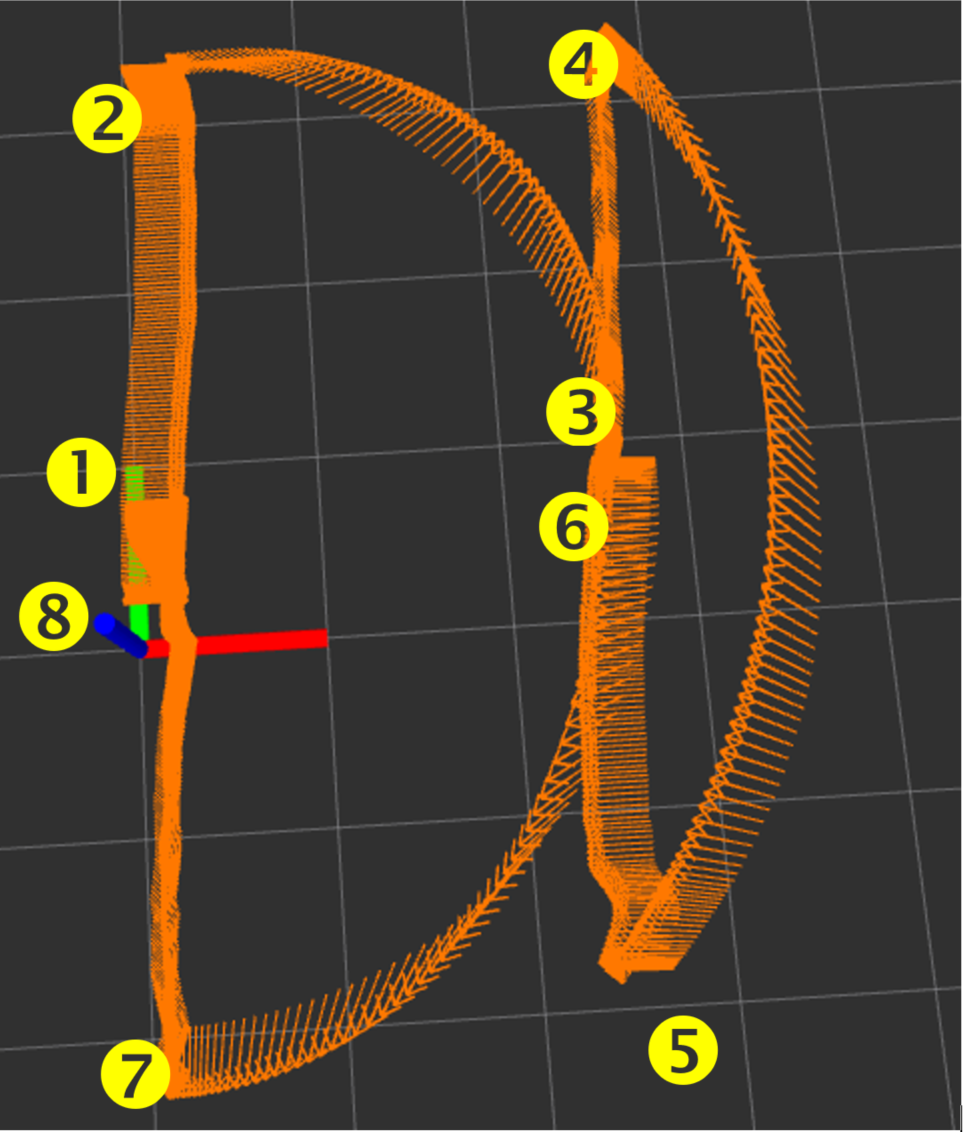
\includegraphics[width=0.4\textwidth]{rot_bug_rviz}
  \caption[Rviz Visualization of Rotational Distortion]{An Rviz visualization of PTAM's rotation defect. This image was created by moving the cart in a 3~m square pattern, turning 90\textdegree\ CCW at each corner.}
  \label{fig:rot_bug_rviz}
\end{wrapfigure}

The experiments chosen to test the system's effectiveness were influenced largely by the known capabilities and limitations of the ROS PTAM implementation\footnote{From here on, ``PTAM'' refers to the particular ROS implementation of PTAM used in the experiments, not to the algorithm in general.}. In previous exploratory experiments\footnote{Performed both by the author and by various other parties at NASA Langley, where the experiments described here took place.}, PTAM was frequently shown to lose tracking\footnote{``Tracking'' here refers to current pose knowledge.} during large rotations. PTAM is particularly susceptible to losing tracking during \textit{pure} rotations, in which the camera rotates in place without translational motion. Worse, whenever PTAM undergoes a rotation, it interprets this as an arc-like motion, regardless of whether any translation took place.

Figure~\ref{fig:rot_bug_rviz} shows PTAM's susceptibility to losing tracking during rotation. This Rviz\footnote{A ROS visualization utility. \url{http://wiki.ros.org/rviz}} visualization was produced by moving the cart in a square trajectory and turning the cart by 90 degrees at each corner. In the figure, the vehicle's trajectory is traced out by a series of orange arrows representing the vehicle's $x$-axis. The vehicle started at the origin (Point~1), then moved forward (in the $+y$ direction) in a straight line to Point~2. At Point~2, the cart was rotated counterclockwise in place by 90 degrees, producing the arc between Points~2 and 3. At this point, the cart was pointed in the $-x$ direction. As the figure shows, this arc extends \textit{opposite} the camera's true direction of travel. After rotating 90 degrees, the vehicle moved in a straight line in the $-x$ direction (Point~3 to Point~4), then rotated again by 90 degrees such that the cart was pointed in the $-y$ direction (Point~4 to 5). Again, the arc goes backward from the actual direction of travel, but this time its length is much greater. This was caused by rotating the vehicle at a higher speed than during the first turn, meaning that this rotation defect is velocity-dependent. From Point~5, the vehicle moves in the $-y$ direction to Point~6, rotates 90 degrees counterclockwise (Point~6 to 7), and then moves in a straight line back to a point near the origin (Point~8).

The trajectory plotted in Figure~\ref{fig:rot_bug_rviz} is vastly distorted. A trusting observer might surmise from the image that the vehicle moved in a pattern resembling two uppercase D's, as opposed to the square pattern traced out in reality. This rotation-translation defect in the ROS PTAM implementation is pervasive and prevents PTAM from being of any real use during rotation. For this reason, the experiments detailed in the next section were carefully performed without rotating the mobile test stand.

\begin{wrapfigure}{l}{0.4\textwidth}
  \centering
    \includegraphics[width=0.4\textwidth]{sensor_mount_vicon}
  \caption[Sensor Mount Instrumented with Retroreflectors]{Close-up view of the sensor mount instrumented with retroreflector balls.}
  \label{fig:sensor_mount_vicon}
\end{wrapfigure}

In other preliminary experiments, anomalous behavior was discovered in PTAM's $z$-position output. Over long translations, the vehicle's estimated altitude could be seen rising erroneously the farther the vehicle moved from the origin. Figure~\ref{fig:bowl-shaped_world} shows a trajectory traced out by moving the test stand several meters to the left and right of the origin in a straight line. In profile, the visualized trajectory is clearly curved. This ``bowl-shaped'' trajectory would seem to arise from lens distortion not properly eliminated by PTAM. PTAM's calibration procedure was repeated several times to try to solve this problem but the distortion persisted. The mvBlueFOX camera has a wide-angle lens with a 150\textdegree\ field of view. During the calibration procedure, camera parameters were computed that, according to the ROS PTAM documentation, were well within acceptable limits for a wide-angle lens. Nevertheless, the aberrant measurements continued.

\begin{figure}[H]
  \centering
    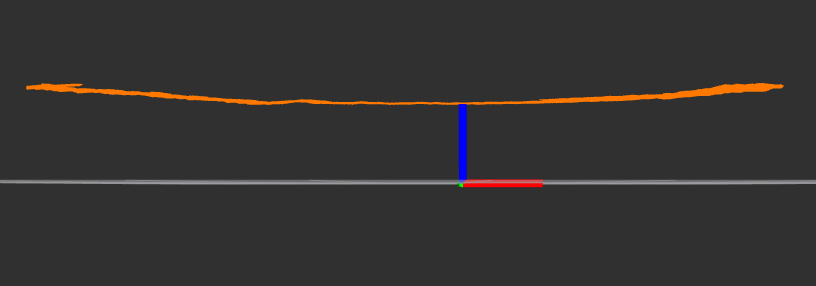
\includegraphics[width=0.9\textwidth]{bowl-shaped_world}
  \caption[Rviz Visualization of Translational (Lens) Distortion]{An Rviz visualization of the ``bowl-shaped'' world seen by PTAM during a long translational motion. This image was created by translating the mobile test stand 3--4~meters in the $+x$ direction and then translating back 4--5~meters past the origin in the $-x$ direction.}
  \label{fig:bowl-shaped_world}
\end{figure}

\section{Experimental Procedures}

\begin{wrapfigure}{r}{0.4\textwidth}
  \centering
    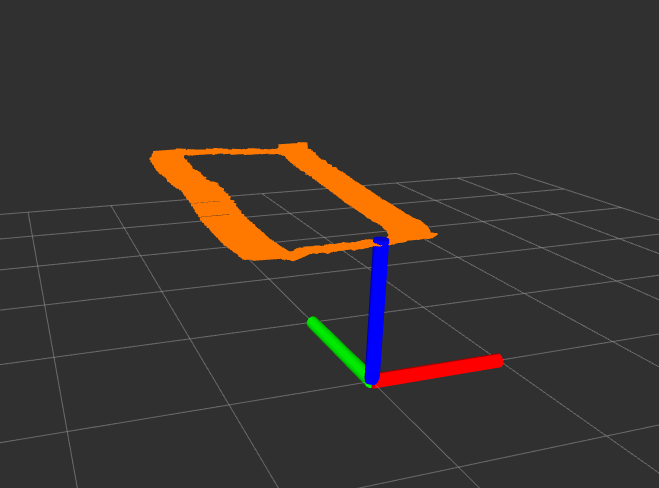
\includegraphics[width=0.4\textwidth]{good_box_5_cropped}
  \caption[Rviz Visualization of a Box Pattern Trajectory]{An Rviz visualization of a box pattern trajectory.}
  \label{fig:good_box}
\end{wrapfigure}

Two experiments were designed to characterize the UKF framework's effectiveness in various regimes of motion. The first experiment was a ``long walk'' in which the mobile test stand was translated in a straight line for several meters along the $y$-axis. This test was designed to characterize the effect of lens distortion on PTAM's $z$-position output, as discussed previously. In the second experiment, the mobile test stand was moved in a rectangular ``box'' pattern (Figure~\ref{fig:good_box}) to determine the system's efficacy in planar motions indicative of hovering flight. Both experiments took place on a level floor to capture more accurately any $z$-directional distortion. Because of the rotation-translation coupling defect found in PTAM, the mobile test stand was moved carefully in each experiment such that it would undergo minimal rotation and thus accurately capture translational motion.

Prior to each trial of each experiment, PTAM was initialized according to the procedure outlined in the documentation. To initialize the algorithm, the camera was placed parallel to the floor at a distance of one meter and then perturbed by 10\% of the distance to the floor (that is, 10~cm). This perturbation tells PTAM its distance to the planar surface in view and thus initializes the map. This initialization procedure was performed by releasing the linear bearing brake (Figure~\ref{fig:sensor_mount_bottom}) on the sensor mount and sliding the mount along the aluminum rail, using the attached adhesive ruler to perturb the camera by exactly 10~cm. After perturbing the camera, the brake was tightened, and the data recording began.

\begin{wrapfigure}{r}{0.5\textwidth}
        \centering
        \includegraphics[width=0.5\textwidth]{sensor_mount_bottom}
        \caption{Bottom view of sensor mount.}
        \label{fig:sensor_mount_bottom}
\end{wrapfigure}

For each long walk trial, the mobile test stand was moved forward in the $+y$ direction by 4--6~meters, being carefully to perturb the stand as little as possible along the $x$-axis. Some amount of lateral instability was unavoidable, however, due to the nature of the floor on which these trials were performed. The rubber tiles covering the floor of the testing area concealed a number of power cables for nearby computers, presenting small ``bumps'' over which the test stand had to pass. These bumps caused uneven left--right perturbations to the test stand, which, though minor in magnitude, proved to be noticeable in post processing (see Chapter~\ref{ch:Exp_Results}). When the test stand had been pushed to the end of the long walk segment, it was then pulled backward in the $-y$ direction until it had approximately returned to the origin.

For the box pattern trials, the mobile test stand was first moved forward in the $+y$ direction by 2.5 to 3~meters. Then, without rotating, the test stand was pushed leftward in the $-x$ direction by approximately 1~meter. The test stand was then pulled backward in the $-y$ direction by 2.5 to 3~meters, returning approximately to $y = 0$. Finally, the test stand was pushed to the right ($+x$) to return to the origin.

\clearpage
\section{Materials}
\subsection{Computation and Sensing}
\begin{enumerate}
\item One (1) MatrixVision mvBlueFOX-MLC Camera\footnote{\url{https://www.matrix-vision.com/USB2.0-single-board-camera-mvbluefox-mlc.html}}
\item One (1) 1044\_0 PhidgetSpatial Precision 3/3/3 High Resolution IMU\footnote{\url{http://www.phidgets.com/products.php?product_id=1044}}
\item One (1) Hewlett-Packard Spectre x360 Convertible Laptop 13-ac076nr\footnote{\url{http://store.hp.com/us/en/pdp/hp-spectre-x360---13-ac076nr}}
\item Two (2) male Mini USB 2.0 to male USB Type A cables
\end{enumerate}
\subsection{Mobile Test Stand}
\begin{enumerate}
\item One (1) Oklahoma Sound PRC200 Premium Presentation Cart\footnote{\url{http://www.oklahomasound.com/products/product-category/single/?prod=9}}
\item One (1) 3D-printed Sensor Mount
\item Two (2) 4" C-Clamps
\item One (1) 1.2-meter 80/20\textsuperscript{\textregistered}~Inc.\ 1515 Rail\footnote{\url{https://8020.net/1515.html}}
\item One (1) 15 Series ``L'' Handle Linear Bearing Brake Kit\footnote{\url{https://8020.net/6800.html}}
\item One (1) $\frac{5}{16}$-18 $\times$ 0.687" Black FBHSCS (Screw)\footnote{\url{https://8020.net/shop/3320.html}}
\item Two (2) Slide-In Economy T-Nuts\footnote{Also available at \url{https://8020.net/shop/3320.html}}
\item Three (3) 1" Vicon Infrared Retroreflector Balls
\item Two (2) $\frac{1}{2}$" Vicon Infrared Retroreflector Balls
\item One (1) 0.7-meter Length of $\frac{1}{8}$"-thick Carbon Fiber Tube
\end{enumerate}
\pagebreak
\chapter{Experimental Results}

\section{Long Walk Trials}

Figures~\ref{fig:longWalk1_xyz}--\ref{fig:longWalk5_xyz} plot the vehicle's $x$-, $y$-, and $z$-coordinates over time. These plots demonstrate that the UKF's pose estimates were able to track the vehicle's $y$-position accurately over the length of each experimental trial. The plots also show that the UKF pose estimates exhibit aberrant behavior causing the vehicle's $z$-position to rise the farther the vehicle moves from the origin. The shaded region in Figure~\ref{fig:longWalk1_xyz} clearly highlights this behavior. The vehicle's altitude as estimated by the UKF rises steadily to a maximum of about 1.4~meters, although in truth the vehicle's altitude was constant throughout. The vehicle's maximum vertical error coincides with its maximal displacement from $\left( 0,\ 0,\ 0 \right)$. 

\begin{figure}
  \centering
    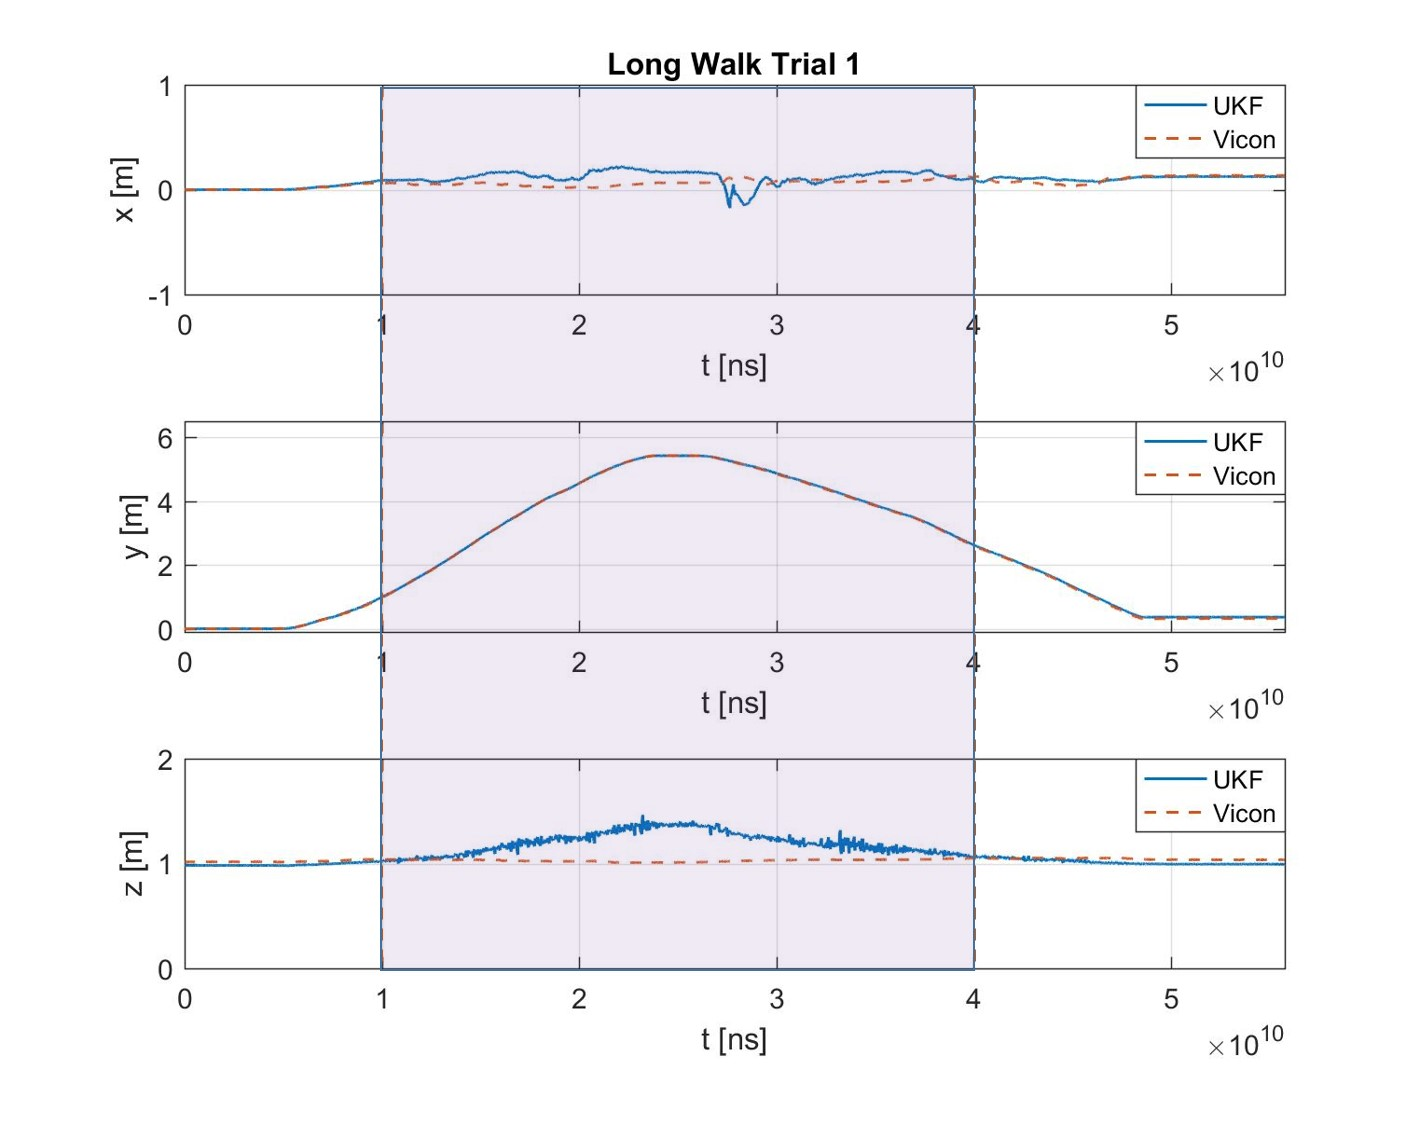
\includegraphics[width=\textwidth]{longWalk1_xyz}
  \caption[Long Walk Trial 1]{Long Walk Trial 1 coordinate plots. The shaded region highlights aberrant behavior coinciding with maximal displacement from the origin.}
  \label{fig:longWalk1_xyz}
\end{figure}

\begin{figure}
  \centering
    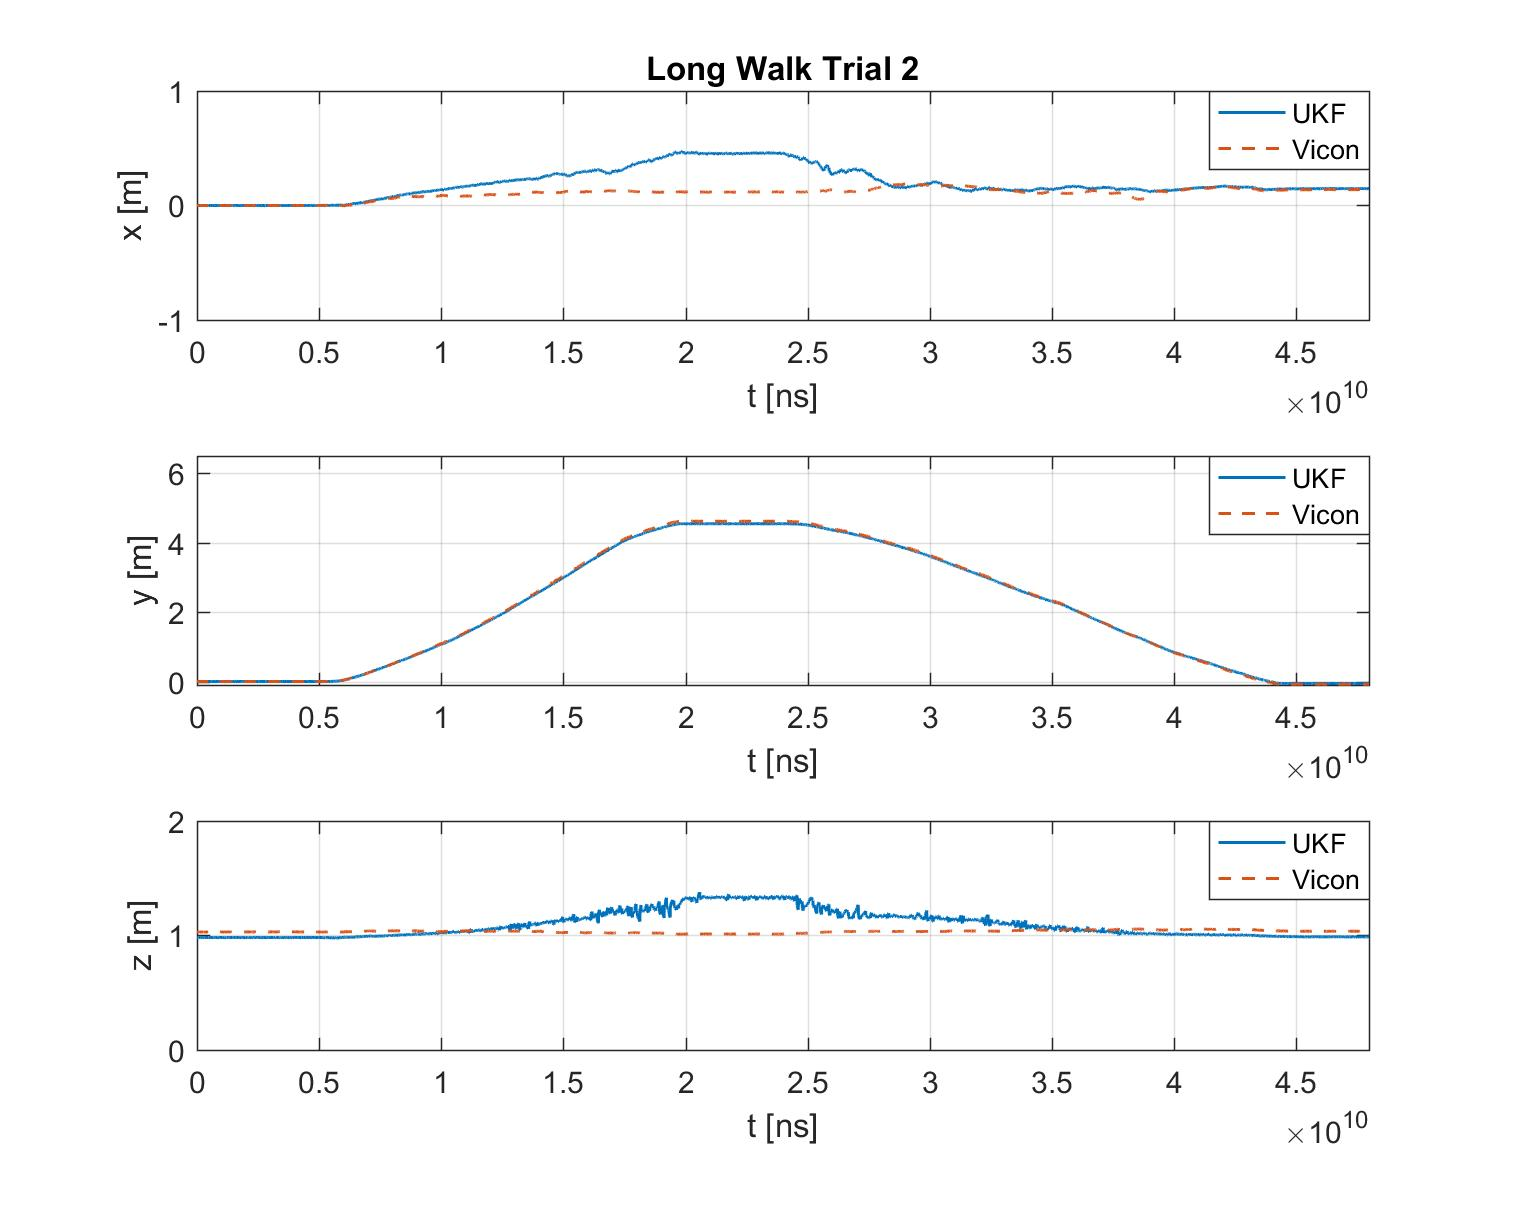
\includegraphics[width=\textwidth]{longWalk2_xyz}
  \caption[Long Walk Trial 2]{Long Walk Trial 2 coordinate plots.}
  \label{fig:longWalk2_xyz}
\end{figure}

\begin{figure}
  \centering
    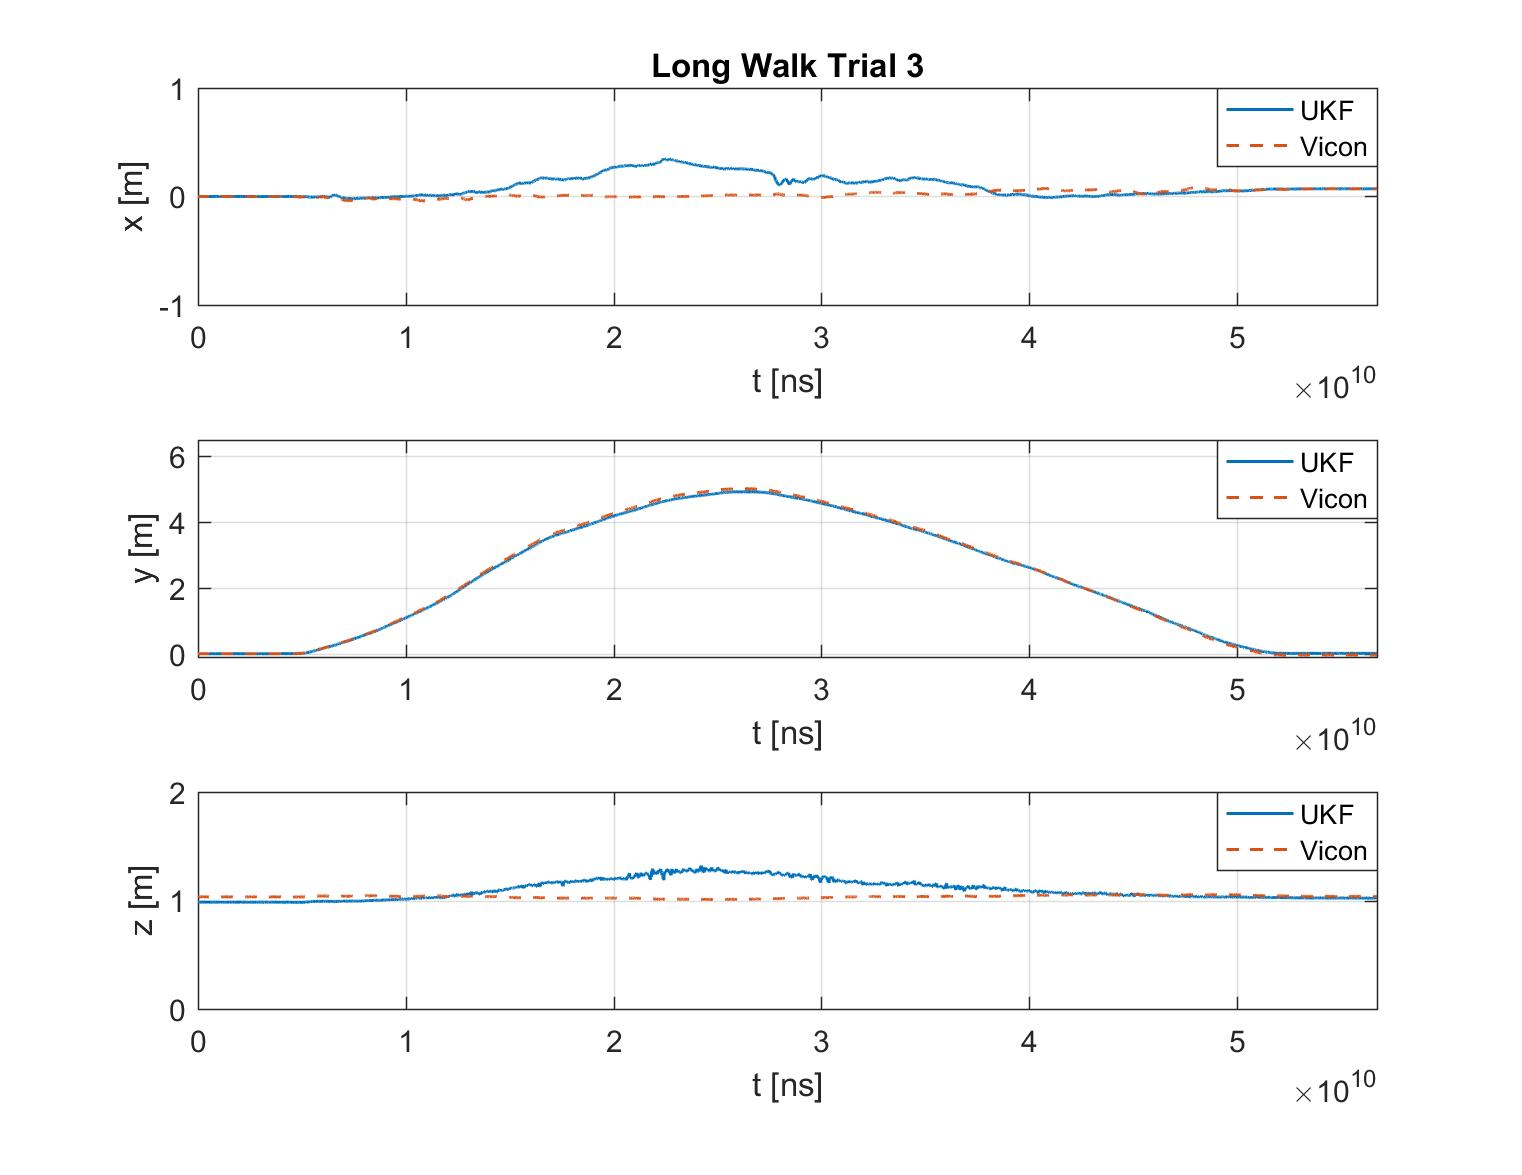
\includegraphics[width=\textwidth]{longWalk3_xyz}
  \caption[Long Walk Trial 3]{Long Walk Trial 3 coordinate plots.}
  \label{fig:longWalk3_xyz}
\end{figure}

\begin{figure}
  \centering
    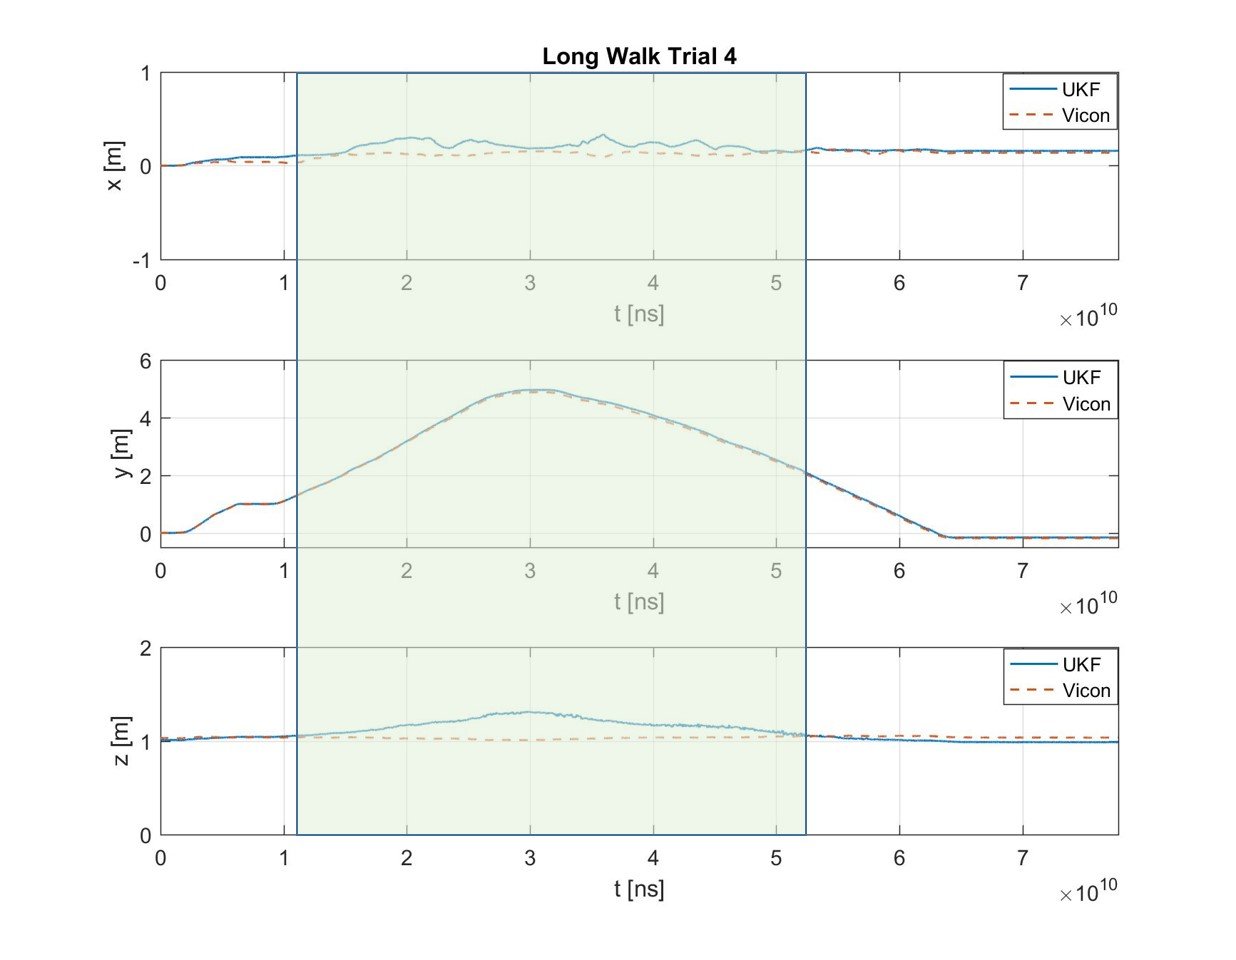
\includegraphics[width=\textwidth]{longWalk4_xyz}
  \caption[Long Walk Trial 4]{Long Walk Trial 4 coordinate plots.}
  \label{fig:longWalk4_xyz}
\end{figure}

\begin{figure}
  \centering
    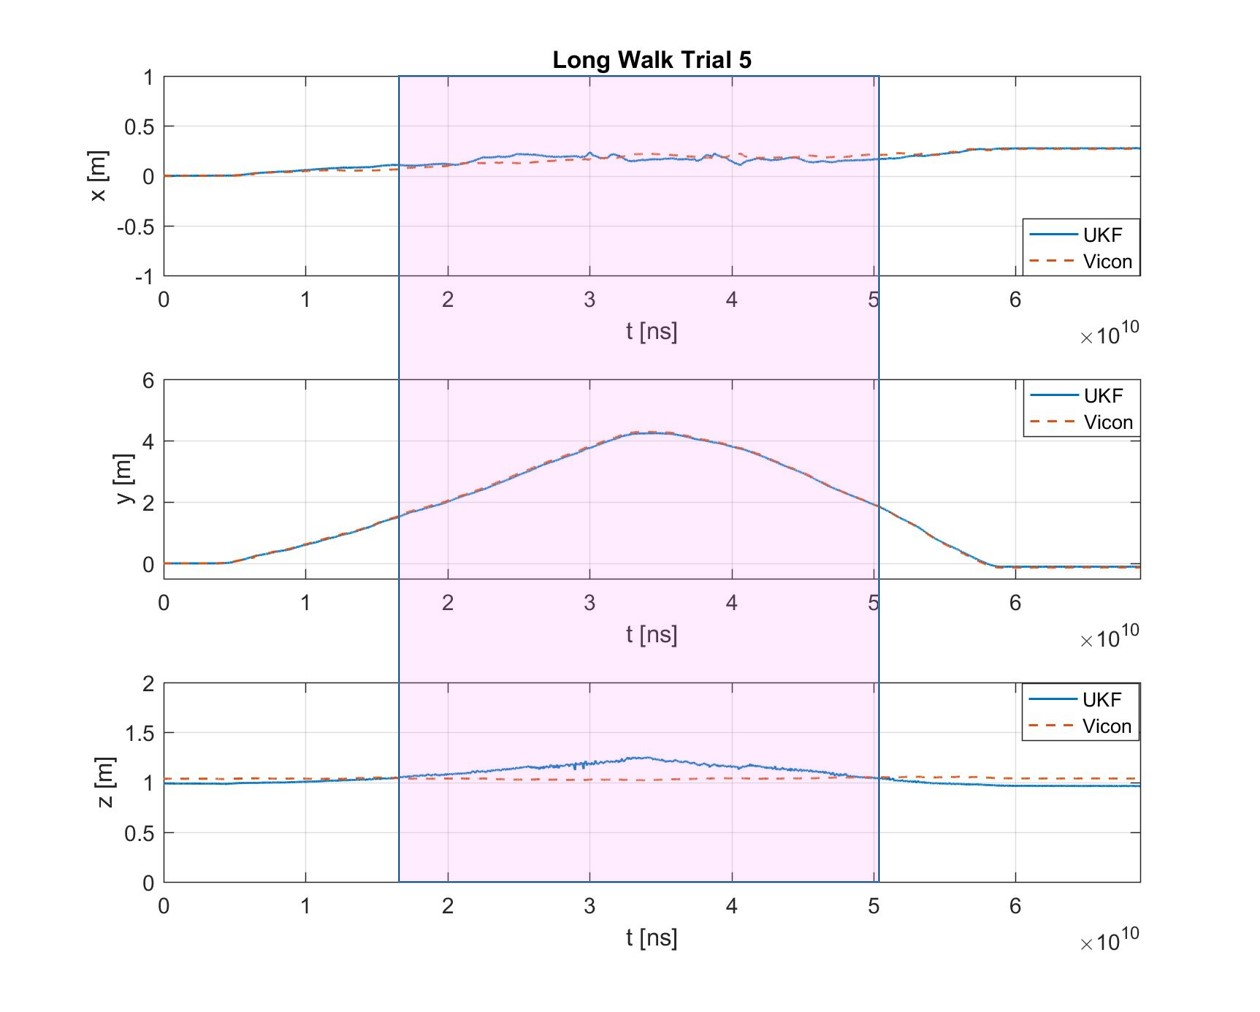
\includegraphics[width=\textwidth]{longWalk5_xyz}
  \caption[Long Walk Trial 5]{Long Walk Trial 5 coordinate plots.}
  \label{fig:longWalk5_xyz}
\end{figure}

\section{Box Pattern Trials}

Figures~\ref{fig:box1_2d}--\ref{fig:box5_3d} plot the estimated and measured trajectories of the mobile test stand during all five box pattern trials. \todo{more}

\clearpage

% Box 1
\begin{figure}[p]
  \centering
    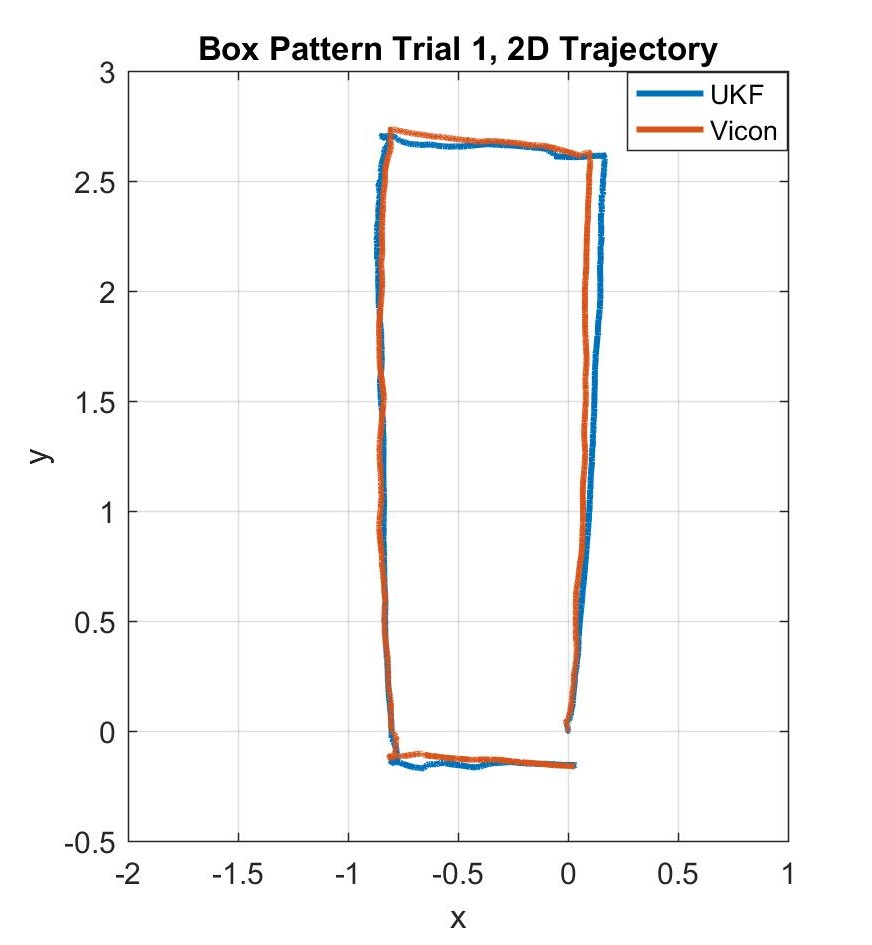
\includegraphics[height=0.6\textwidth]{box1_2d}
  \caption[Box Pattern Trial 1 2D Trajectory]{Box Pattern Trial 1 2D Trajectory.}
  \label{fig:box1_2d}
\end{figure}
\begin{figure}[p]
  \centering
    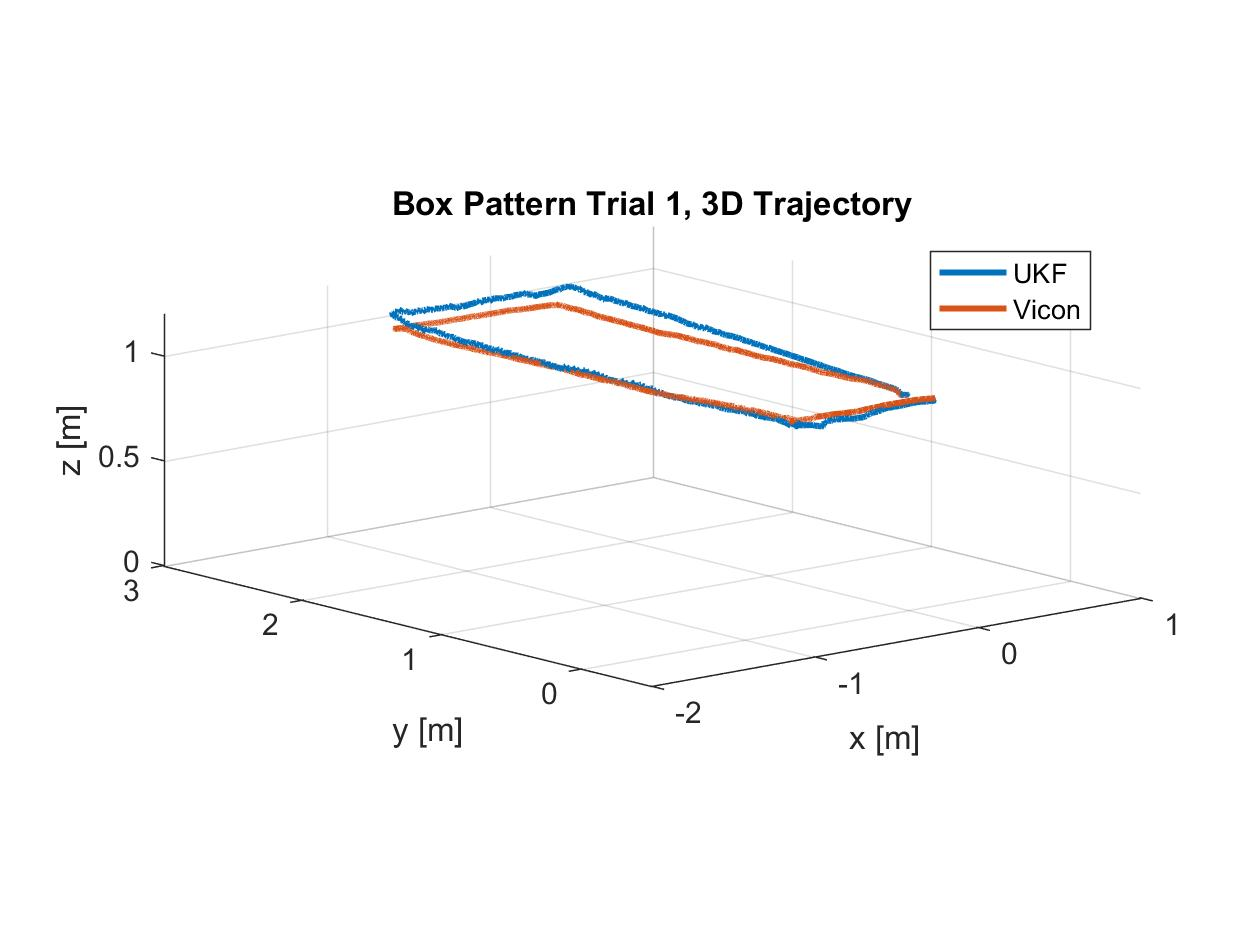
\includegraphics[height=0.7\textwidth]{box1_3d}
  \caption[Box Pattern Trial 1 3D Trajectory]{Box Pattern Trial 1 3D Trajectory.}
  \label{fig:box1_3d}
\end{figure}
\clearpage

% Box 2
\begin{figure}[p]
  \centering
    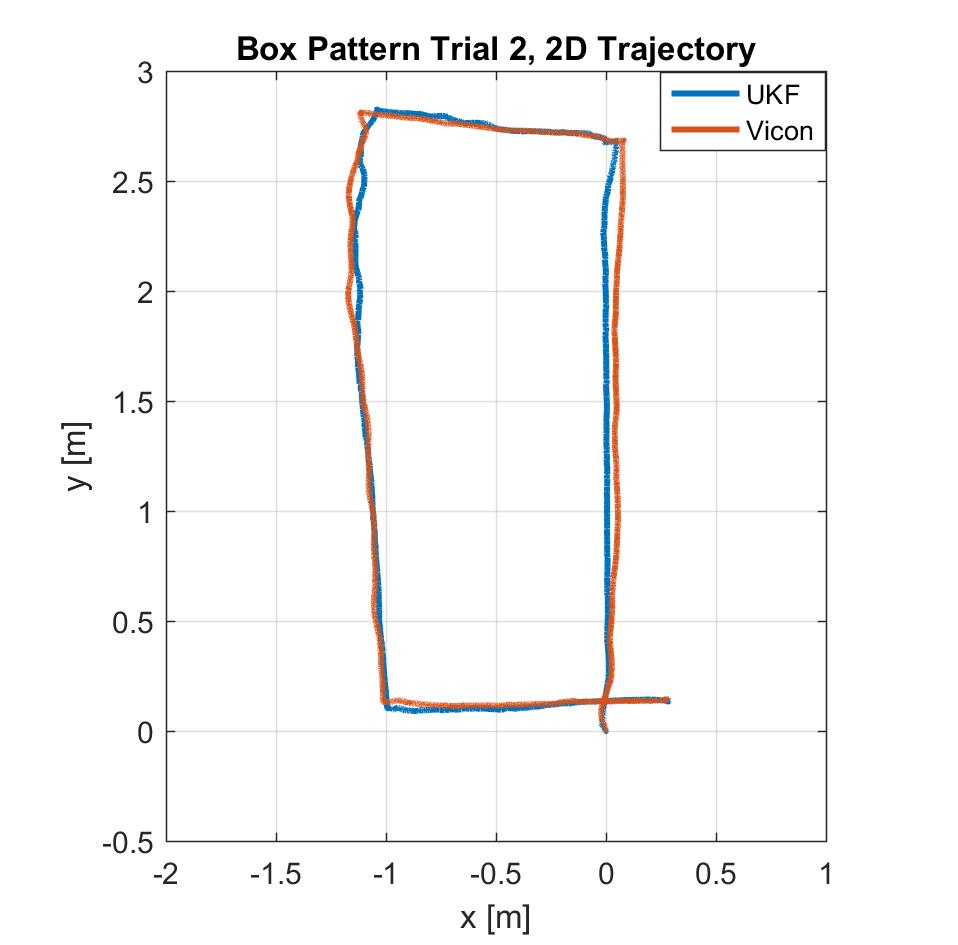
\includegraphics[height=0.6\textwidth]{box2_2d}
  \caption[Box Pattern Trial 2 2D Trajectory]{Box Pattern Trial 2 2D Trajectory.}
  \label{fig:box2_2d}
\end{figure}
\begin{figure}[p]
  \centering
    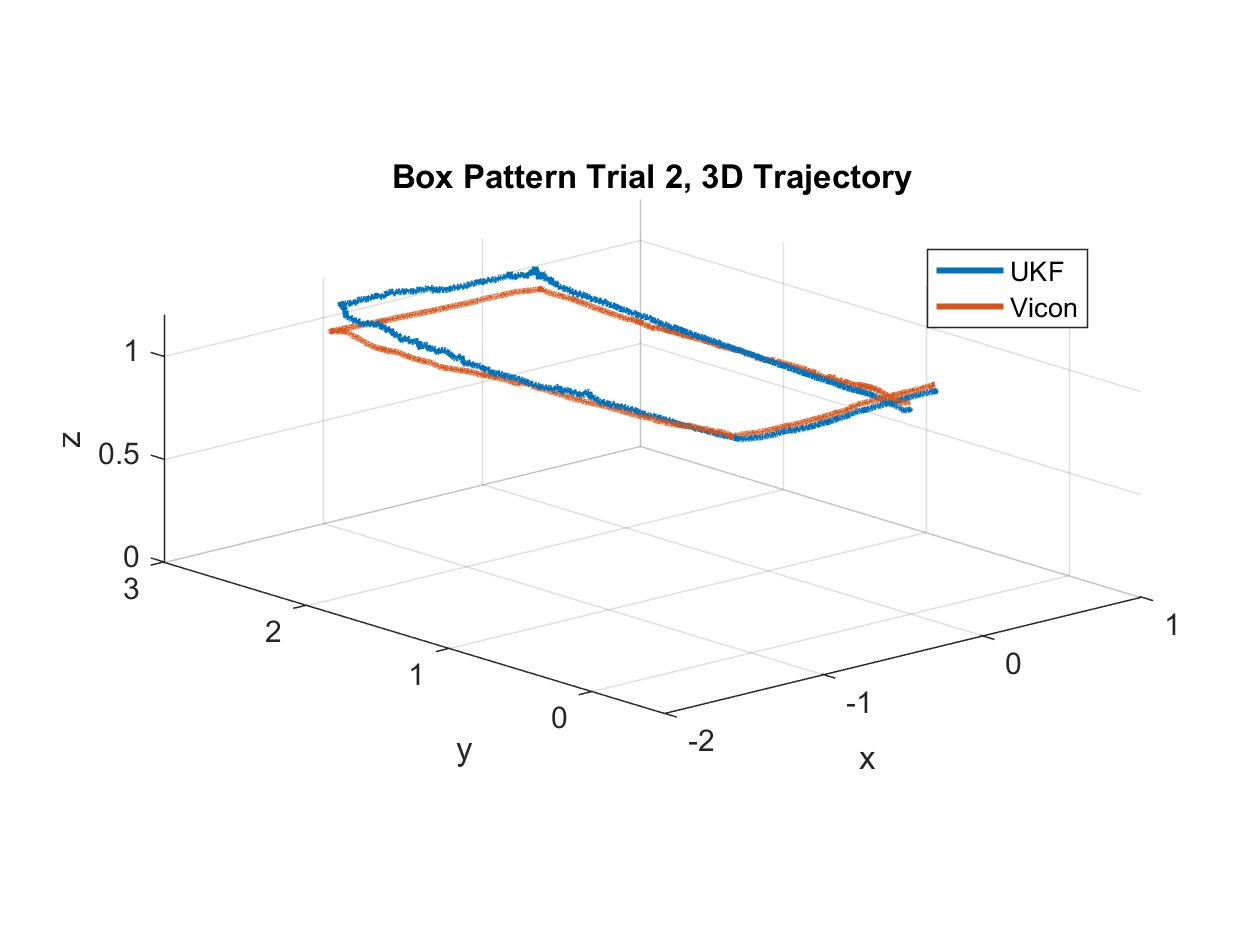
\includegraphics[height=0.7\textwidth]{box2_3d}
  \caption[Box Pattern Trial 2 3D Trajectory]{Box Pattern Trial 2 3D Trajectory.}
  \label{fig:box2_3d}
\end{figure}
\clearpage

% Box 3
\begin{figure}[p]
  \centering
    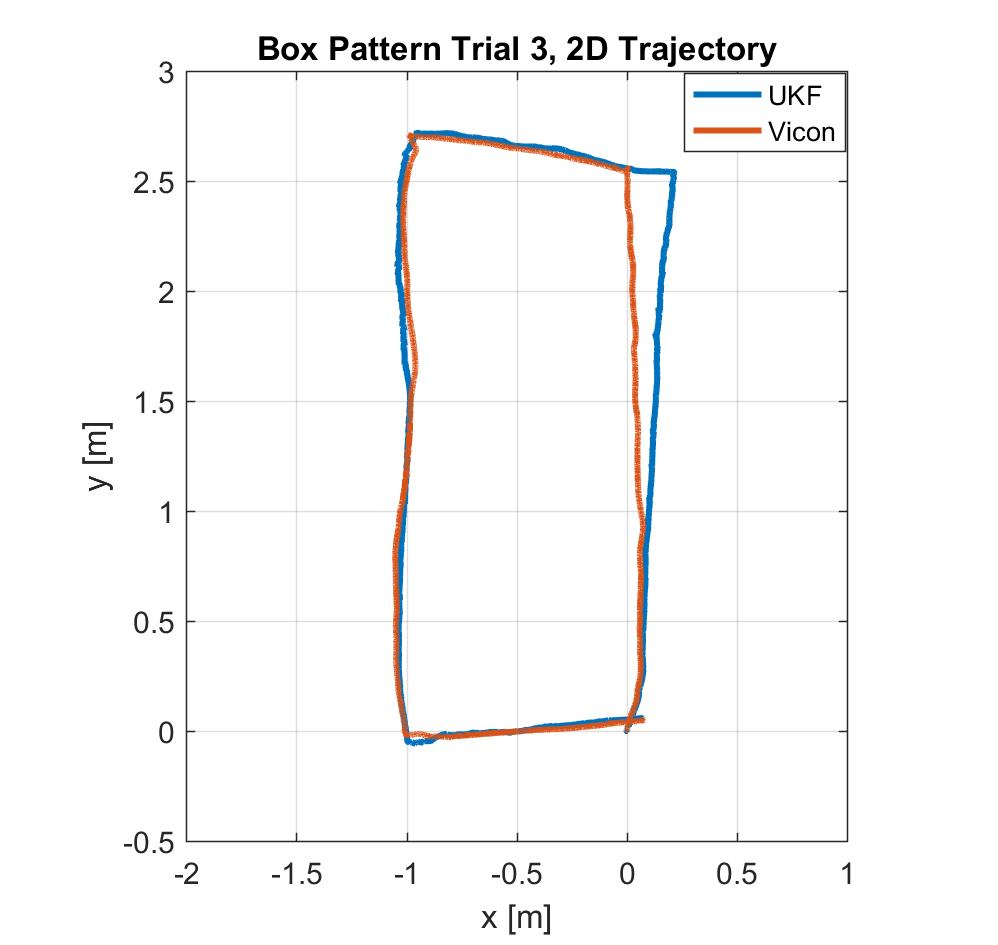
\includegraphics[height=0.6\textwidth]{box3_2d}
  \caption[Box Pattern Trial 3 2D Trajectory]{Box Pattern Trial 3 2D Trajectory.}
  \label{fig:box3_2d}
\end{figure}
\begin{figure}[p]
  \centering
    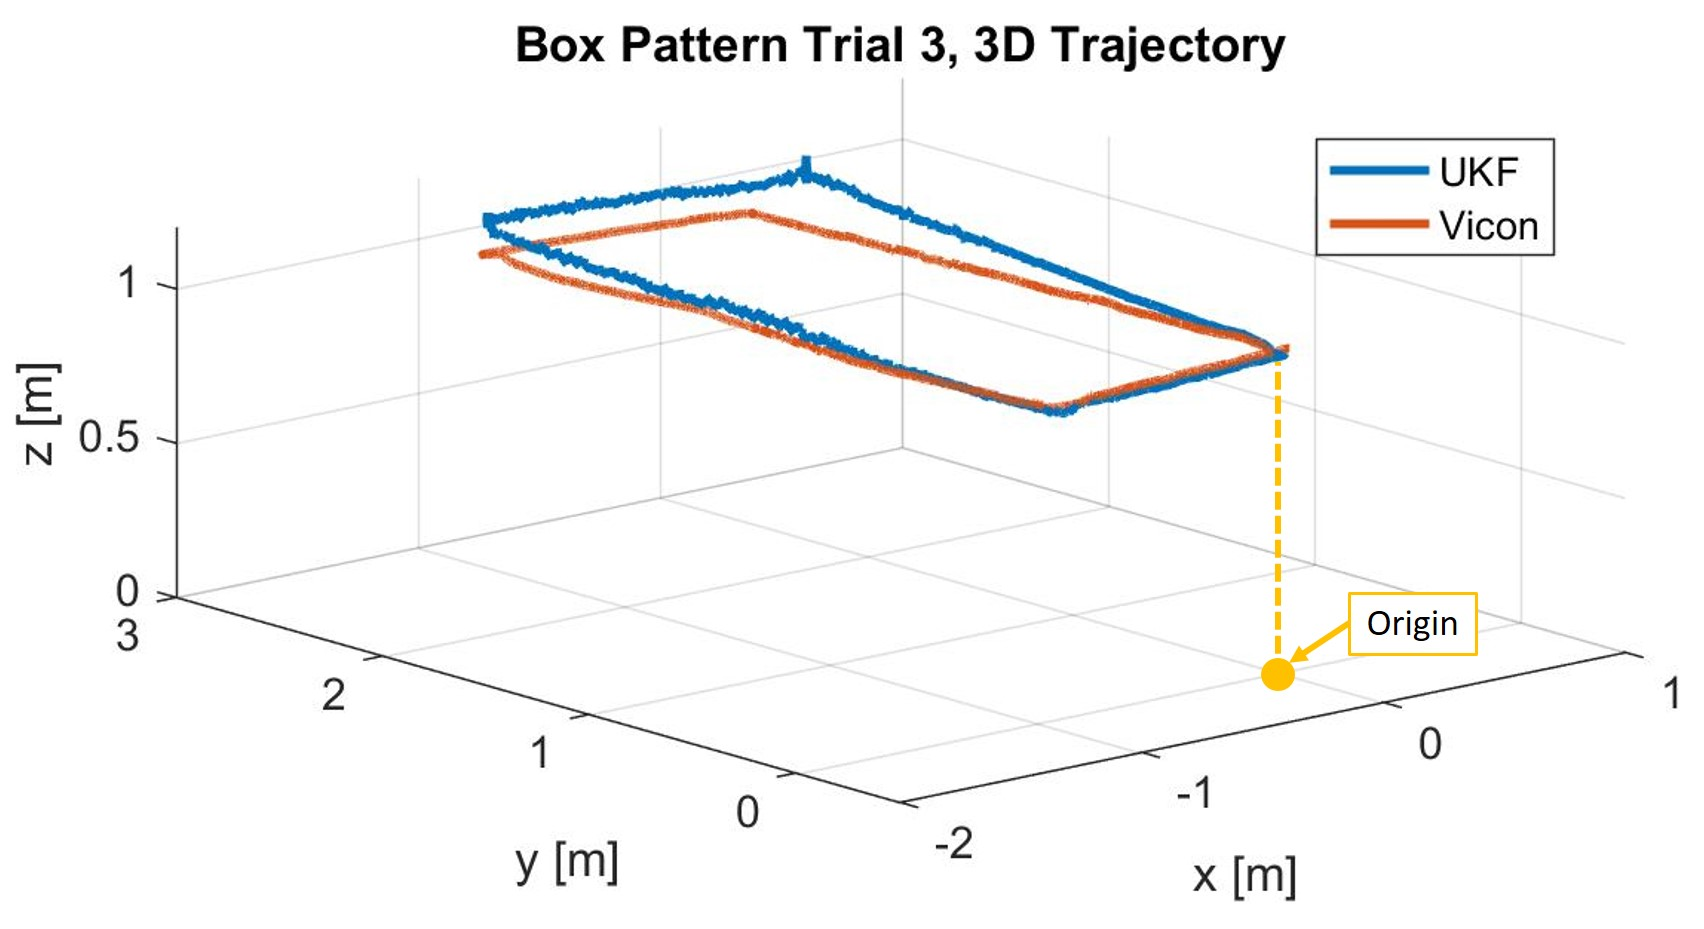
\includegraphics[height=0.7\textwidth]{box3_3d}
  \caption[Box Pattern Trial 3 3D Trajectory]{Box Pattern Trial 3 3D Trajectory.}
  \label{fig:box3_3d}
\end{figure}
\clearpage

% Box 4
\begin{figure}[p]
  \centering
    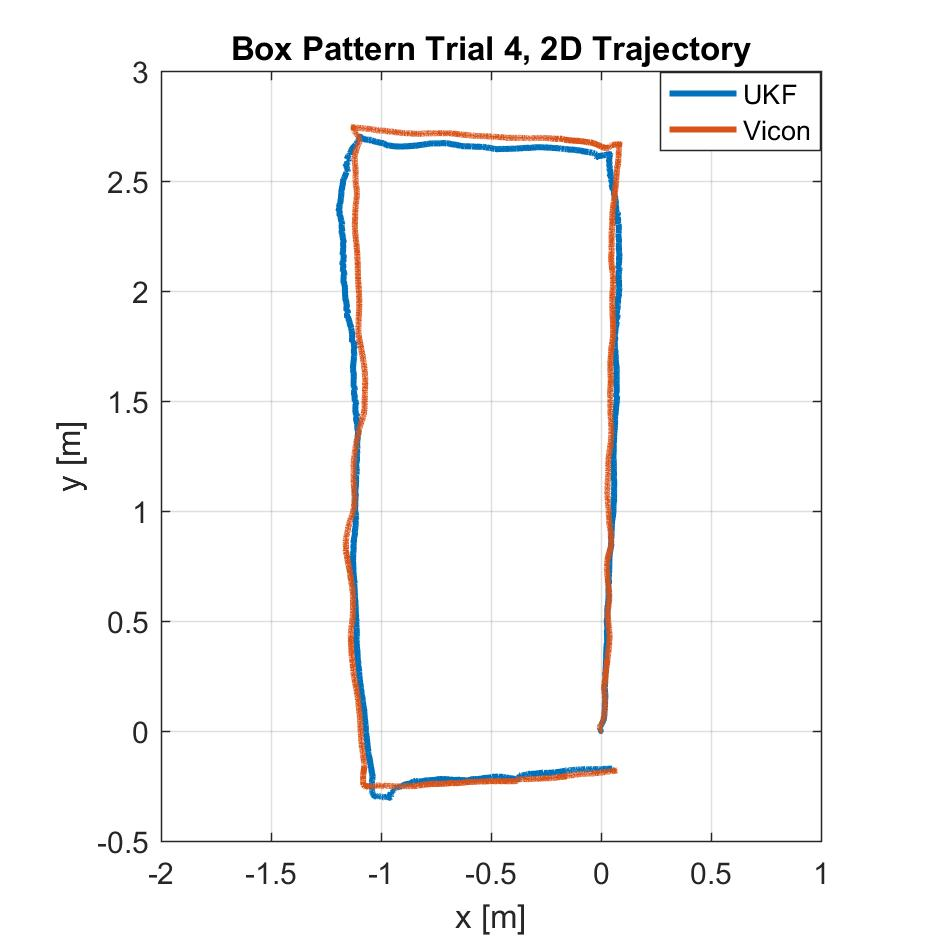
\includegraphics[height=0.6\textwidth]{box4_2d}
  \caption[Box Pattern Trial 4 2D Trajectory]{Box Pattern Trial 4 2D Trajectory.}
  \label{fig:box4_2d}
\end{figure}
\begin{figure}[p]
  \centering
    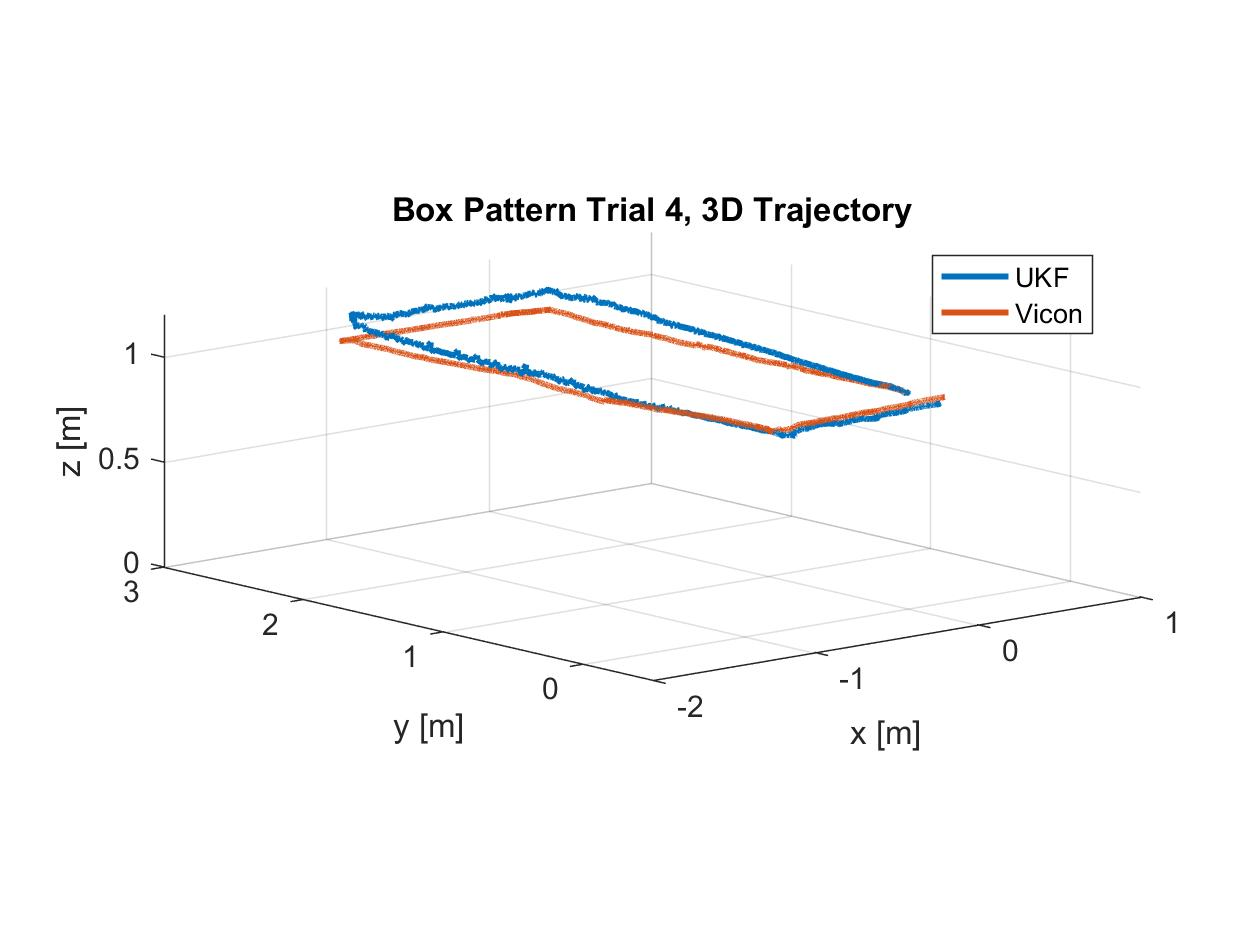
\includegraphics[height=0.7\textwidth]{box4_3d}
  \caption[Box Pattern Trial 4 3D Trajectory]{Box Pattern Trial 4 3D Trajectory.}
  \label{fig:box4_3d}
\end{figure}
\clearpage

% Box 5
\begin{figure}[p]
  \centering
    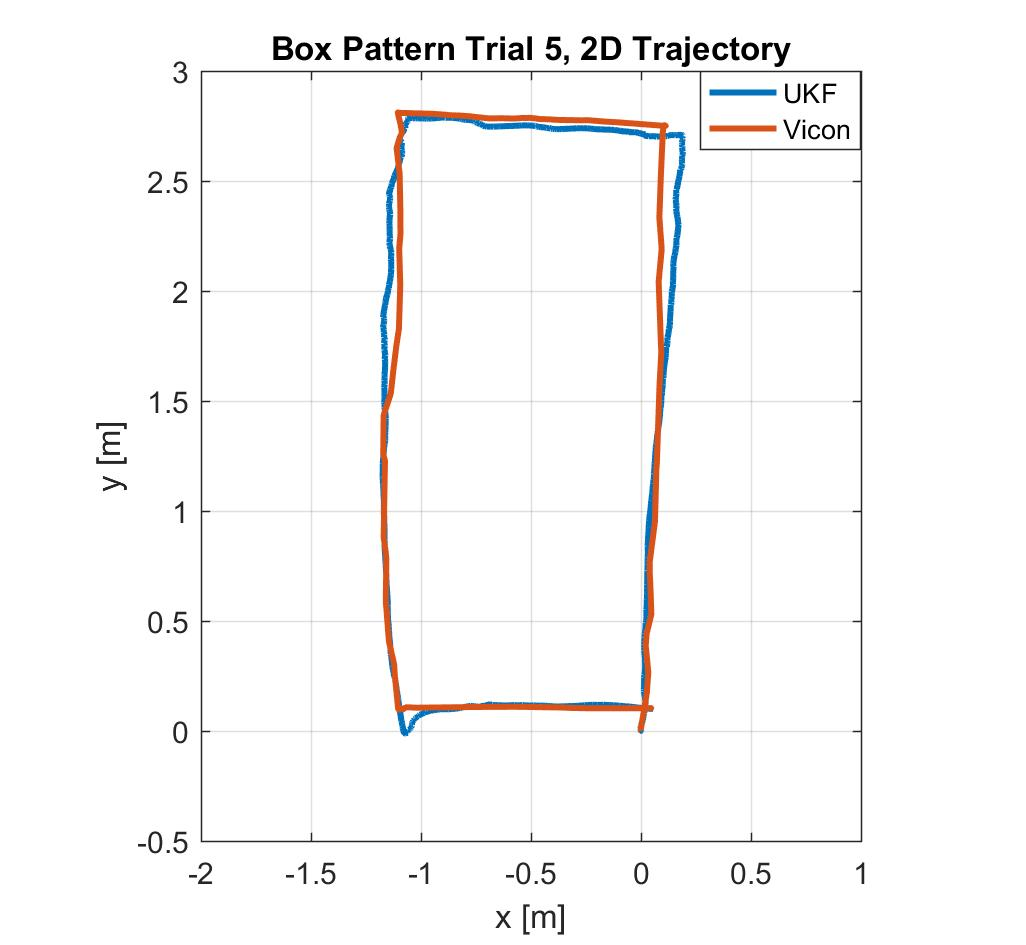
\includegraphics[height=0.6\textwidth]{box5_2d}
  \caption[Box Pattern Trial 5 2D Trajectory]{Box Pattern Trial 5 2D Trajectory.}
  \label{fig:box5_2d}
\end{figure}
\begin{figure}[p]
  \centering
    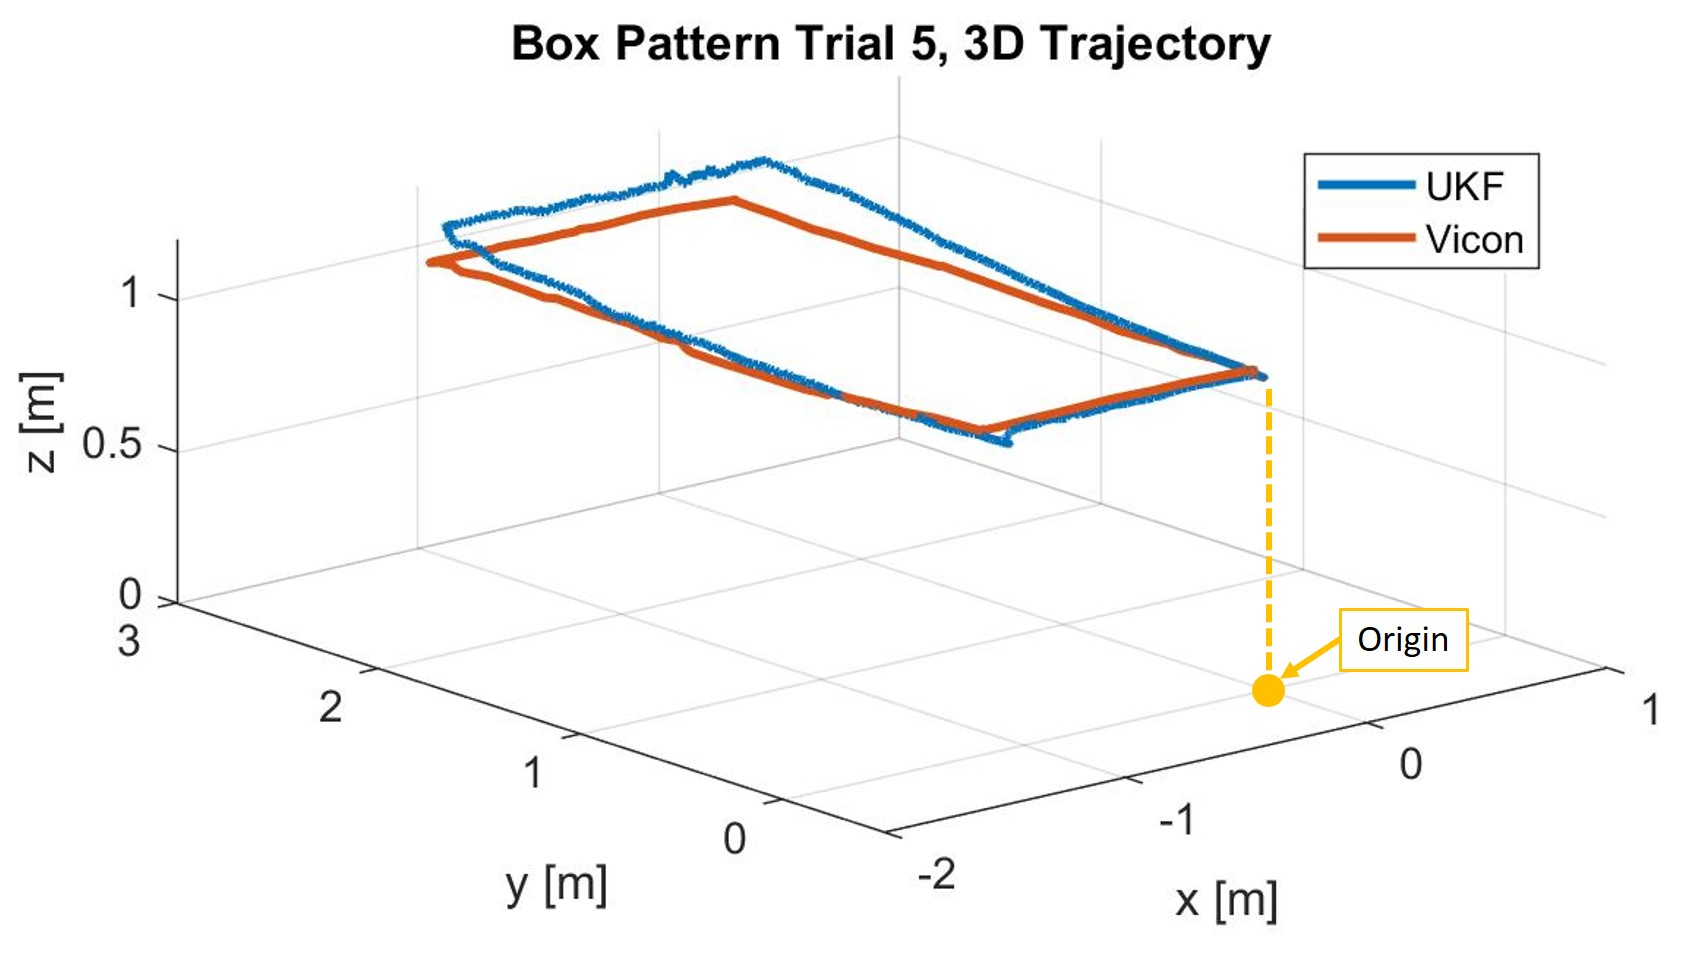
\includegraphics[height=0.7\textwidth]{box5_3d}
  \caption[Box Pattern Trial 5 3D Trajectory]{Box Pattern Trial 5 3D Trajectory.}
  \label{fig:box5_3d}
\end{figure}
\clearpage

\section{Post Processing}

Two data streams were recorded using the \texttt{rosbag}\footnote{\url{http://wiki.ros.org/rosbag}} recording utility: the pose messages published by \texttt{kalman\_sense} and the pose messages published by Vicon. To determine the effectiveness of the UKF framework in estimating the position of the vehicle, positional errors were computed per the following relations:
%
\begin{align}
\varepsilon_{x} &= | x_{\text{Vicon}} - x_{\text{UKF}} | \\
\varepsilon_{y} &= | y_{\text{Vicon}} - y_{\text{UKF}} | \\
\varepsilon_{z} &= | z_{\text{Vicon}} - z_{\text{UKF}} |
\end{align}
%
These positional errors were computed over the \todo{finish}


\chapter{Conclusions and Future Work}

\section{Conclusions}

In the course of this research, we have developed an algorithm for fusion of IMU and SLAM data for localization of a small aircraft capable of hovering flight. We have presented not only an Unscented Kalman Filter formulation for this purpose, but also two corrective measures for maintaining quaternion continuity and deriving velocity measurements from pose readings to maintain numerical stability in the filter's output. We have also presented software implementation details related to the creation of a ROS package performing this fusion algorithm and described a number of architectural traits of this package encouraging and allowing for the adaptation of this work to systems other than small rotorcraft.

This work is largely motivated by the confluence of increased computing power and increased payload capacity for small UAS. The system developed in this thesis is meant to empower the roboticist researcher with a general state estimation framework useful for modeling a wide range of systems with arbitrary levels of fidelity. The experiments detailed in Chapters~\ref{ch:Exp_Design} and \ref{ch:Exp_Results} deployed the system in an indoor navigation scenario to characterize its behavior in a realistic environment where GPS would never be available as a backup sensing modality. In box pattern tests, the system consistently maintained a mean total position error of less than 10~cm with maximal errors never exceeding 25.96~cm. By these performance metrics, the UKF framework is more accurate than today's smartphone-grade GPS receivers and on par with similar sensor fusion systems detailed in Chapter~\ref{ch:Prior_Work}.

Nevertheless, the system faces several critical challenges. The PTAM implementation used during the experiments suffers from a number of serious defects. This PTAM implementation exhibits aberrant $z$-position estimates over flat terrain, erroneously conflates rotations with translations, and appears not to eliminate lens distortion. These defects severely limit the possible use cases for the system, assuming the same PTAM implementation is used. For effective use in non-laboratory scenarios, the vehicle would have to fly in pure translation (that is, without substantial rotations). Though this may seem like an odd requirement, modern hobby-grade autopilots, such as the Pixhawk, already allow for precisely this type of flight.

Perhaps the more stringent requirement on this system is that it be used in environments with ample visual geometry. The SLAM algorithm used in experimentation was susceptible to losing tracking if the density of visible features was not sufficiently high. This would be a necessary condition for any SLAM/VO algorithm, meaning that the system can only be deployed in areas with plenty of high-contrast features (and sufficient lighting by which to see them).

With all of this being said, the UKF framework developed here still represents a useful jumping-off point for further work. Future developments in this area (explored in detail in the next section) will likely revolve around increasing accuracy and robustness, the two principle challenges of any navigation system. Even the much-glorified Global Positioning System is not without its systemic faults and environmental limitations. Because of its generality, this work could be applied to great effect in numerous state estimation scenarios. Beyond rotorcraft and fixed-wing airplanes, this UKF framework could be adapted for use with spacecraft, surface vessels, undersea vehicles, and automobiles. Due to increasing demand for intelligent systems and unmanned vehicles of many varieties, it is likely that research in this area will continue for decades to come. In any case, the emphasis will likely remain on higher accuracy and greater robustness. With the growing trend of miniaturization and the increasing density of human populations, the need for ever more precise localization will always be present.

\section{Future Work}

\subsection{System Improvements}

Experimentation with the \texttt{kalman\_sense} ROS package has revealed a number of areas for improvement. Speaking generally, the system needs enhancements to improve accuracy and to become more robust with respect to sensor malfunction. Further development of this work likely would center on three main areas:
\begin{enumerate}
    \item Integration of new sensors,
    \item Improvements for current sensors, and
    \item Refinements to the underlying algorithm.
\end{enumerate}
Modifications to any or all of these areas would produce a marked improvement to the system in terms of both accuracy and robustness. For maximal effectiveness in adverse conditions, the system's sensors would need to be both individually robust and collectively redundant, so that complementary sensors could compensate for the loss of another sensor's information.

\subsubsection{Integration of New Sensors}
The accuracy and robustness of the system could be augmented by the integration of additional sensors, including but not limited to, the following:
\begin{enumerate}
    \item One or more GPS receivers (particularly Real Time Kinematic\footnote{\url{https://en.wikipedia.org/wiki/Real_Time_Kinematic}} GPS),
    \item A pressure altimeter,
    \item A 3-axis magnetometer,
    \item One or more laser rangefinders,
    \item One or more forward-facing cameras (preferably depth cameras, such as RGB-D),
    \item One-dimensional, multi-dimensional, or scanning LIDAR\footnote{``Light Detection and Ranging,'' \url{https://en.wikipedia.org/wiki/Lidar}}.
\end{enumerate}

\begin{comment}
\begin{center}
\begin{tabular}{ m{0.25\textwidth} | m{0.65\textwidth} }
 GPS & Position (and orientation, if using multiple receivers for differential GPS) \\
 Pressure Altimeter & Altitude \\
 3-Axis Magnetometer & Heading angle \\
 Ventral Laser Rangefinder & Altitude \\
 Longitudinal/Lateral Laser Rangefinders & Distance to obstacles \\
 Forward-Facing Camera & Roll angle, distance to obstacles \\
 1D LIDAR & Similar to Laser Rangefinder \\
 Multi-dimensional/Scanning LIDAR & Full 3D map of surroundings, distance to obstacles
\end{tabular}
\end{center}
\end{comment}

We previously mentioned work from the GRASP Lab (\cite{Shen2011}) that demonstrated the efficacy of similar UKF frameworks in indoor-outdoor transitions and in navigating confined spaces using an expanded suite of sensors. In the case where more than one sensor is used to observe a given vehicle state variable, those multiple sensors check one another and can even perform real-time, in-air calibration. The system developed in this thesis has the advantage of being hardware-minimal in that it depends on only two sensors (the IMU and the ventral camera), but this convenience comes at the cost of robustness because either sensor presents a single point of possible failure. Moreover, the sensors have no overlap. Neither can observe any of the states observed by the other. This eliminates the possibility of checking one sensor against the other. Introducing a ventral laser rangefinder or pressure altimeter would allow for much more precise measurement of the vehicle's altitude and would allow for in-flight re-initialization of any metric SLAM/VO algorithm.

With the exception of certain sensors such as scanning LIDAR, which can cost tens of thousands of dollars, and RTK-GPS, which often falls in the same price range, these proposed new sensors would be inexpensive additions to the vehicle. Given the sophistication of current miniaturized sensors, it is not unreasonable to expect sub-meter or centimeter-level position accuracy from vehicles weighing fewer than fifteen pounds (including a substantial sensor payload) and costing less than 20,000~USD. It has been the case for a number of years now that meter-level accuracy could be taken for granted with ``toy'' quadcopters using only MEMS\footnote{``Microelectromechanical systems,''\\ \url{https://en.wikipedia.org/wiki/Microelectromechanical_systems}} IMUs and sub-\$100 GPS receivers. The trend of miniaturization has made more and more sensors of better and better quality increasingly available in the weight- and cost-constrained world of aerial robotics. A variety of inexpensive off-the-shelf autopilots, such as the Pixhawk~2.1\footnote{\url{http://www.proficnc.com/}}, already boast triple-redundant IMUs and support for multiple GPS modules. Many of the hardware integration challenges that once plagued hobbyists and researchers have been resolved by engineering developments stemming from popular demand for user-friendly drones.

The organization of the \texttt{kalman\_sense} package's code base is such that the integration of new sensors would require only the addition of new callback functions and ROS subscribers, as opposed to a full redesign or major edits to the existing code. Further, a new SLAM or VO algorithm could also be used in lieu of PTAM, allowing an ``apples-to-apples'' comparison of different visual localization algorithms. For example, Donavanik et~al.\ \cite{Donavanik2016} have identified a new algorithm known as ORB-SLAM \cite{Mur-Artal2015} as a promising candidate for robust SLAM, already implemented in ROS. Because of ROS's sophisticated ecosystem of interoperable packages and message formats, any pose sensor employing the same message type as PTAM could plug in to \texttt{kalman\_sense} in a matter of seconds.

Much of the design thinking that went into the \texttt{kalman\_sense} package was focused on this particular possibility. The aircraft of the future will be vehicles laden with a vast suite of heterogeneous sensors, the outputs of which would, at any given time, be used not only for inner-loop and outer-loop flight control, but also for self-calibration, real-time diagnostics, and operator telemetry. Future UAVs will be akin to floating laboratories, mobile arrays of cutting-edge measurement systems allowing remote sensing over areas of several square miles.

\subsubsection{Improvements for Current Sensors}

For improved pose measurements, a more robust implementation of PTAM could be written and the same experiments could be repeated for comparison. PTAM's rotation errors and inability to eliminate lens distortion constitute severe limitations to its effectiveness in small UAS navigation. Moreover, if a rewritten formulation were able to interface with a downward-facing rangefinder, the initialization process could be eliminated altogether. The drawback is that making these changes would require a major software rewrite, a project that could be feasibly undertaken only by an experienced team of computer vision researchers and software developers. The mere cost in terms of both time and labor would likely make this an unappealing proposition, especially if other ready-made SLAM/VO algorithms were available to serve as PTAM replacements.

Processing power will also be central to the system's effectiveness during deployment on a real aircraft. This research is in many ways the product of recent advances in computing power. The advent of miniature desktop computers, such as the Intel~NUC\footnote{``Next Unit of Computing,'' \url{https://en.wikipedia.org/wiki/Next_Unit_of_Computing}}, as well as power-efficient Graphics Processing Units\footnote{\url{https://en.wikipedia.org/wiki/Graphics_processing_unit}} (GPUs) has made a new frontier of estimation and localization algorithms easily accessible for the first time in the UAV world. A simple and generally inexpensive approach to augmenting the \texttt{kalman\_sense} system would thus be the inclusion of top-of-the-line lightweight computing hardware. With modern onboard computers, even the need for cross-platform code compilation (so-called ``transpiling'') is eliminated because these computers employ the same x86 architecture used by most software developers.

\subsubsection{Refinements to the Underlying Algorithm}

The UKF formulation itself presents another set of opportunities for improvement. In particular, better process and measurement noise modeling would allow for increased accuracy. As described previously, the noise covariance matrices used during the experiments were only rough, static models meant to overestimate the Gaussian noise in the system. In practice, it would be better to replace these with time-varying matrices with terms more closely matching the intrinsic parameters of the system. Due to the high degree of coupling between state variables and the fundamental nonlinearity of the process model, this type of work was considered to be outside the scope of my thesis. In the future, however, a better $\mathbf{Q}$ matrix could be determined, perhaps by application of autocovariance and system identification methods. Moreover, any new sensor integrated into the system would require its own $\mathbf{R}$ matrix detailing its particular idiosyncrasies. With this done, attention could then be turned to tuning the $\mathbf{Q} / \mathbf{R}$ ratio of each sensor, thus making the system even more faithful to known sensor parameters. With more sensors, self-calibration techniques such as those employed in \cite{Weiss2012} could also be implemented to avoid the process of reinitializing one or more sensors in mid-air.

\subsection{Future Experiments}

Using a SLAM/VO algorithm that addresses pure rotation and lens distortion would be the easiest and most cost effective way to improve the system. Testing different visual localization algorithms would thus be an appealing avenue of inquiry. It would behoove the researcher to characterize the system's behavior under the same conditions that caused the PTAM-based implementation to fail. In particular, experiments that include pure rotations and longer translations, as well as simulated flight movement over uneven but otherwise virtually unchanging terrain would mimic real-world flight missions more closely and provide a more holistic understanding of the system's effectiveness. Additionally, mounting the sensor suite on the underside of a UAV would allow for the collection of real-world flight data, which could shed light on the system's speed limits and behavior in the presence of in-flight vibrations.

After integrating new sensors, new experiments could be devised to characterize the system's effectiveness during sensor blackouts---for example, during an indoor-outdoor transition after integrating a GPS receiver. Experiments such as this could then inform the design of heuristic models for recognizing sensor degradation and perhaps even consensus-based estimation strategies. 

\subsection{System Applications}

Applications for this system are wide-ranging, spanning virtually every conceivable use for a small drone. The following is a non-exhaustive list of possible applications:
\begin{enumerate}
    \item Mapping and 3D reconstruction of structures and topography,
    \item Emergency response,
    \item Infrastructure inspection,
    \item Autonomous package delivery, and
    \item Military/defense solutions.
\end{enumerate}
What all of these applications have in common is the need for robust localization. In each of the above scenarios, losing GPS could cause a crash. In such an event, the vehicle itself would pose a real threat to bystanders and property. Moreover, in the case of military aircraft, the vehicle could be captured by hostile forces.

\subsubsection{Mapping and 3D Reconstruction}

Growing demand for so-called ``precision agriculture'' has brought with it the need to map large areas of cropland at a high speed, with a low cost point. In the past, this need has been met by using satellite imagery and human-captured photography. With the arrival of low-cost drones, this work has been offloaded to aerial robots. Outfitted with specialized sensors such as hyperspectral cameras\footnote{\url{https://en.wikipedia.org/wiki/Hyperspectral_imaging}}, small UAS are now able to provide minute-by-minute coverage of large expanses of land. More interesting still, these robots can be outfitted with reservoirs of pesticide or fertilizer and deployed to spray individual plants autonomously. It is in roles such as this that high-accuracy robust localization becomes a necessity. The accuracy required for precision agriculture can be provided by utilizing the sensor fusion techniques discussed in this thesis.

The surfaces of buildings and other structures can be mapped in a similar fashion, given the appropriate sensors and the right framework by which to fuse them. 3D reconstruction has become popular among real estate agents, safety inspectors, and other parties with a vested interest in precise 3D renderings of large geometries. In this case, the aircraft must be able to localize itself precisely in order to take full advantage of onboard sense-and-avoid technologies. The ability of the aircraft to estimate its position is crucial to its ability to map hard-to-reach areas and maintain stable flight. Sensor fusion systems shine when GPS and other sensors are inevitably compromised by various environmental factors.

\subsubsection{Emergency Response}

UAS technologies have become a desirable tool for first responders in many parts of the world. The ability to deploy a UAV to survey forest fires or search for missing persons has been a game changer for law enforcement and emergency response teams. In the case of looking for survivors of a natural disaster, the requirements for an effective vehicle system are accurate localization and overall robustness. Vehicles sent into disaster areas will have to be able to navigate in sensor-compromising environments, sometimes at substantial speed. This use case highlights the need for redundant sensors and intelligent, failure-resistant sensor fusion.

\subsubsection{Infrastructure Inspection}

Infrastructure inspection is similar in several respects to 3D mapping. In both cases, small drones are preferable to manned aircraft because of their low cost, high maneuverability, and ease of use. In recent years, governments and private corporations have taken an interest in using small aircraft to automate the inspection of many types of infrastructure, including the following:
\begin{enumerate}
    \item Power lines,
    \item Oil rigs,
    \item Gas pipelines,
    \item Railroads, and
    \item Buildings.
\end{enumerate}
UAVs are an obvious ally to companies servicing most types of static infrastructure. Inspecting miles of wires or railroad track is a task well-suited to today's UAVs, which commonly ship with intuitive flight planning software. Operators---even those who have no experience flying remote-control aircraft---are now able to program missions and deploy drones with ease. The aircraft are able to survey miles of infrastructure regardless of conditions on the ground, such as flooding, ill-maintained roads, or wild animals. Operators with First-Person View (FPV) hardware can watch video streaming live from the aircraft as if they were onboard themselves. The need for robust localization here is obvious: the UAV cannot inspect anything to which it cannot navigate. Operating in the wilderness may require flying below the forest canopy or under natural overhangs that could block GPS reception. The same is true in urban environments, where tall buildings create so-called ``urban canyons'' which compromise GPS effectiveness. Large metal structures can also distort magnetometry readings and thus undermine the aircraft's ability to maintain its heading. In any case, UAVs used for large-scale inspections will be dependent upon intelligently combined sensing modalities.

\subsubsection{Autonomous Package Delivery}

A number of organizations, most notably Amazon\footnote{\url{https://www.amazon.com/Amazon-Prime-Air/b?node=8037720011}}, have made big bets on drones as the future of delivery services. The task of delivering goods to individual homes is no trifling matter. American homes come in all shapes and sizes and are surrounded by numerous structures and natural obstacles that could endanger a delivery aircraft and, by extension, the people and property nearby. Moreover, any drone delivery service would have to be predicated upon the ability of the UAV to land with sub-meter accuracy. Delivery drones will have to land precisely in cluttered environments amid dynamic obstacles. Visual sensing will be extremely important for identifying safe landing zones, avoiding power lines and fences, and surmounting other environmental challenges. GPS alone will not be enough to guide the vehicle safely in every conceivable circumstance. 

\subsubsection{Military/Defense Solutions}

Perhaps the most obvious application of a UKF fusion framework is in military operations, where precision navigation and robustness to sensor degradation are paramount for protecting soldiers in the field. As of the time of this writing, UAVs have been used in combat for years. However, augmented navigation could still make revolutionary contributions in areas such as
\begin{enumerate}
    \item Robust tracking of friendly and hostile elements,
    \item Remote observation of roads and vehicle-related hazards,
    \item Autonomous deliveries of materiel in-theater, and
    \item Human-machine teaming.
\end{enumerate}
Every combat zone will constitute a hostile environment for UAV operations, especially in the presence of GPS spoofing/jamming technologies. Combat UAVs will have to be able to tolerate multiple simultaneous sensor failures. Moreover, in-theater urban flight operations bring with them all of the same difficulties mentioned above, but with the added challenge of violent enemy interdiction. Robust sensor fusion could automate the task of operational overwatch and provide mission-critical intelligence in a timely manner---but only if the vehicle can localize itself reliably in sensor-hostile environments.
\chapter{Future Work}

\section{Improving \texttt{kalman\_sense}}

Experimentation with \texttt{kalman\_sense} has revealed a number of areas for improvement. Speaking generally, the system needs enhancements to become more accurate and more robust to sensor dropout. Further development of this work would likely center on three main areas:
\begin{enumerate}
\item Integration of new sensors,
\item Improvements for current sensors, and
\item Refinements to the underlying algorithm.
\end{enumerate}
Each of these could produce a marked improvement to the system in accuracy, robustness, or both. Particular use cases, Concepts of Operations (CONOPS), and desired performance metrics would likely drive the selection of which of these areas to tackle.

\subsection{Integration of New Sensors}
The accuracy and robustness of the system could be augmented by the integration of additional sensors, including but not limited to
\begin{enumerate}
\item One or more GPS receivers (particularly Real Time Kinematic\footnote{\url{https://en.wikipedia.org/wiki/Real_Time_Kinematic}} GPS),
\item A pressure altimeter,
\item One or more laser rangefinders,
\item One or more forward-facing cameras (preferably depth cameras, such as RGB-D),
\item One-dimensional, multi-dimensional, or scanning LIDAR\footnote{``Light Detection and Ranging,'' \url{https://en.wikipedia.org/wiki/Lidar}}.
\end{enumerate}
We have previously mentioned work from the GRASP Lab (\cite{Shen2011}) that has demonstrated the efficacy of systems similar to \texttt{kalman\_sense} in indoor-outdoor transitions and in navigating confined spaces with an expanded suite of sensors. In the case where more than one sensor can be used to observe a given vehicle state variable, those multiple sensors can be used to check one another and even perform real-time, in-air calibration. The system developed in this thesis has the advantage of being hardware-minimal in that it depends on only two sensors (the IMU and ventral camera), but this convenience comes at the cost of robustness as either sense presents a single point of failure. Moreover, the sensors have no overlap in that neither can observe any of the states observed by the other. This eliminates the possibility of checking one sensor against the other with high confidence. Introducing a ventral laser rangefinder or pressure altimeter would allow for much more precise measurement of the vehicle's altitude and would allow for in-flight re-initialization of any metric SLAM/VO algorithm.

With the exception of certain sensors such as scanning LIDAR, which can cost tens of thousands of dollars, and RTK-GPS, which often falls in the same price range, these proposed new sensors would be inexpensive additions to the vehicle. Given the sophistication of current miniaturized sensors, it is not unreasonable to expect sub-meter or centimeter-level position accuracy from vehicles weighing fewer than fifteen pounds (including a substantial sensor payload) and costing less than 20,000~USD. It has been the case for a number of years now that meter-level accuracy could be taken for granted with ``toy'' quadcopters using only MEMS\footnote{\url{https://en.wikipedia.org/wiki/Microelectromechanical_systems}} IMUs and sub-\$100 GPS receivers. The trend of miniaturization has made more and more sensors of better and better quality increasingly available in the weight- and cost-constrained world of aerial robotics. A variety of inexpensive off-the-shelf autopilots, such as the Pixhawk~2.1\footnote{\url{http://www.proficnc.com/}}, already boast triple-redundant IMUs and support for multiple GPS modules. Many of the hardware integration challenges that once plagued hobbyists and researchers have been eliminated by popular demand for user-friendly drones.

The organization of \texttt{kalman\_sense}'s code base is such that the integration of new sensors would require only the addition of new callback functions and ROS subscribers, as opposed to a full redesign or any major edits to the existing code. By a similar token, a new SLAM or VO algorithm could also be used in place of PTAM, allowing an ``apples-to-apples'' comparison of different vision algorithms. For example, Donavanik et al.\ (\cite{Donavanik2016}) have identified a new algorithm known as ORB-SLAM (\cite{Mur-Artal2015}) as a promising candidate for robust SLAM, already implemented in ROS. Because of ROS's sophisticated ecosystem of interoperable packages and message formats, any pose sensor employing the same message type as PTAM could plug in to \texttt{kalman\_sense} in a matter of seconds.

Much of the design thinking that went into the design of the \texttt{kalman\_sense} package was focused on this particular possibility. The aircraft of the future are rapidly becoming ``hundred-eyed monsters''---vehicles laden with a vast suite of heterogeneous sensors, the outputs of which are at any given time being used not only for inner-loop and outer-loop flight control but also for self-calibration, real-time diagnostics, and operator telemetry. Future UAVs will be akin to floating laboratories, carrying numerous means of measurement for all manner of self-sensing as well as scientific applications.

\subsection{Improvements for Current Sensors}

For improved pose measurements, a more robust implementation of PTAM could be written and the same experiments could be repeated for comparison. PTAM's rotation errors and inability to eliminate lens distortion pose severe limitations to its effectiveness in small UAS navigation. Moreover, if a rewritten implementation were able to interface to a downward-facing rangefinder, the initialization process could be eliminated altogether. The problem with this is that making these changes would likely require a major rewrite, a project that could only feasibly be undertaken by an experienced team of computer vision researchers and software developers. The mere cost in terms of both time and labor would likely make this an unappealing proposition, especially if other ready-made SLAM/VO algorithms were available to serve as PTAM replacements.

On that same note, the system's processing power could always be augmented through the inclusion of a powerful onboard computer and one or more Graphics Processing Units\footnote{\url{https://en.wikipedia.org/wiki/Graphics_processing_unit}} (GPUs).

\subsection{Refinements to the Underlying Algorithm}





\section{Future Experiments}

\section{System Applications}

\clearpage
\addcontentsline{toc}{chapter}{Bibliography}
\bibliographystyle{ieeetr}
\bibliography{bibliography}

%\appendix
% http://tex.stackexchange.com/questions/49643/making-appendix-for-thesis
%\input{Code_Listing.tex}

\end{document}